\documentclass[12pt, a4paper]{article}
\usepackage{ctex}

\usepackage[margin=1in]{geometry}
\usepackage{
  color,
  clrscode,
  amssymb,
  ntheorem,
  amsmath,
  listings,
  fontspec,
  xcolor,
  supertabular,
  multirow,
  mathtools,
  mathrsfs
}
\definecolor{bgGray}{RGB}{36, 36, 36}
\usepackage[
  colorlinks,
  linkcolor=bgGray,
  anchorcolor=blue,
  citecolor=green
]{hyperref}
\newfontfamily\courier{Courier}

\theoremstyle{margin}
\theorembodyfont{\normalfont}
\newtheorem{thm}{定理}
\newtheorem{cor}[thm]{推论}
\newtheorem{pos}[thm]{命题}
\newtheorem{lemma}[thm]{引理}
\newtheorem{defi}[thm]{定义}
\newtheorem{std}[thm]{标准}
\newtheorem{imp}[thm]{实现}
\newtheorem{alg}[thm]{算法}
\newtheorem{exa}[thm]{例}
\newtheorem{prob}[thm]{问题}
\DeclareMathOperator{\sft}{E}
\DeclareMathOperator{\idt}{I}
\DeclareMathOperator{\spn}{span}
\DeclareMathOperator*{\agm}{arg\,min}
\newcommand{\pr}{\prime}
\newcommand{\tr}{^\intercal}
\newcommand{\st}{\text{s.t.}}
\newcommand{\hp}{^\prime}
\newcommand{\ms}{\mathscr}
\newcommand{\mn}{\mathnormal}
\newcommand{\tbf}{\textbf}
\newcommand{\mbf}{\mathbf}
\newcommand{\fl}{\mathnormal{fl}}
\newcommand{\f}{\mathnormal{f}}
\newcommand{\g}{\mathnormal{g}}
\newcommand{\R}{\mathbf{R}}
\newcommand{\Q}{\mathbf{Q}}
\newcommand{\JD}{\textbf{D}}
\newcommand{\rd}{\mathrm{d}}
\newcommand{\str}{^*}
\newcommand{\vep}{\varepsilon}
\newcommand{\lhs}{\text{L.H.S}}
\newcommand{\rhs}{\text{R.H.S}}
\newcommand{\con}{\text{Const}}
\newcommand{\oneton}{1,\,2,\,\dots,\,n}
\newcommand{\aoneton}{a_1a_2\dots a_n}
\newcommand{\xoneton}{x_1,\,x_2,\,\dots,\,x_n}
\newcommand\thmref[1]{定理~\ref{#1}}
\newcommand\lemmaref[1]{引理~\ref{#1}}
\newcommand\defref[1]{定义~\ref{#1}}
\newcommand\posref[1]{命题~\ref{#1}}
\newcommand\secref[1]{节~\ref{#1}}
\newcommand\equref[1]{(\ref{#1})}
\newcommand\figref[1]{图 \ref{#1}}
\newcommand\corref[1]{推论~\ref{#1}}
\newcommand\exaref[1]{例~\ref{#1}}
\newcommand\algref[1]{算法~\ref{#1}}
\newcommand{\remark}{\paragraph{评注}}
\newcommand{\example}{\paragraph{例}}
\newcommand{\proof}{\paragraph{证明}}


\title{科学计算 笔记}
\author{任云玮}
\date{}

\begin{document}
\lstset{numbers=left,
  basicstyle=\scriptsize\courier,
  numberstyle=\tiny\courier\color{red!89!green!36!blue!36},
  language=C++,
  breaklines=true,
  keywordstyle=\color{blue!70},commentstyle=\color{red!50!green!50!blue!50},
  morekeywords={},
  stringstyle=\color{purple},
  frame=shadowbox,
  rulesepcolor=\color{red!20!green!20!blue!20}
}
\maketitle
\tableofcontents
\newpage
\section{绪论}

\subsection{计算机数值计算基本原理}

\subsubsection{实数的存贮方法}
  \begin{defi}[二进制浮点数系]\footnote{floating Number System}
    实数在计算机内部为\tbf{近似存贮},采用二进制浮点数系
    \[
      F(2,n,L,U)=\{\pm0.\aoneton\times10^m\}\cup\{0\}
    \]
    其中$a_1=1$,$a_i\in\{0,\,1\}$. 指数$m$满足$L\le m\le U$.
    称$n$为其字长,$2$表示采用二进制.
  \end{defi}

  \begin{std}[IEEE]
    $\,$
    \begin{enumerate}
      \item 单精度: $t=24,L=-126,U=127$
      \item 双精度: $t=53,L=-1022,U=1023$
      \item Underflow Limit: $UFL=0.1\times2^L$.
      若$0<x<UFL$,则$\\fl(x)=0$.
      \item Overflow Limit: $OFL=0.11\dots1*2^U$.
      若$x>OFL$,则$\fl(x)=\infty$.
      \item 舍入: 若$UFL\le x\le OFL$,则$\fl(x)$为舍入所得浮点数.
      舍入规则如下:设$x=0.\aoneton\dots\times2^m$. 若$a_{n+1}=1$,
      则$d_t+1$并舍弃其后项;否则直接舍弃其后项.
    \end{enumerate}
  \end{std}

  \begin{defi}[机器精度]
    下仅考虑舍去的情况.
    \[\begin{split}
    x-\fl(x) &= 2^m \times 0.0\dots0a_{n+2}\dots \\
    &=2^m \times [2^{-(t+2)} + 2^{-(t+3)} + \cdots] \\
    &=2^m\times2^{-(t+1)}
    \end{split}\]
    其相对误差满足
    \[
      \frac{x-\fl(x)}{x} < \frac{x-\fl(x)}{0.5\times2^m}=2^{-t}
    \]
    记为$\varepsilon$,称之为机器精度.
  \end{defi}

  \begin{pos}
    \[
      \fl(x)=x(1+\delta),\,\text{其中}\,|\delta|\le\varepsilon
    \]
  \end{pos}

\subsubsection{实数的基本运算原理}
  加法$+$硬件实现$\Rightarrow$四则运算.

  \begin{imp}[$x+y$]
    设$x,\,y$为浮点数,则$x+y$的实现方式如下:
    \begin{enumerate}
      \item 对阶:将指数$m$化为两者中较大者;
      \item 尾数相加;
      \item 舍入;
      \item 溢出分析等……
      \item 结果输出.
    \end{enumerate}
  \end{imp}
  \remark
    由$\fl(x)+\fl(y)=x(1+\delta_x)+y(1+\delta_y)$可知,当一个
    大数与一个小数相加时,小数有可能被忽略,所以应当避免大数小数间的相加.

\newpage
\subsection{误差的来源与估计}

\subsubsection{误差的来源}
 \begin{enumerate}
  \item 模型问题. 例:近似地球为球体来计算.
  \item 测量误差. 例:测量地球半径时的误差.
  \item 方法误差(截断误差).
  例:对于$y=\f(x)$,求$\f(x^*)$时使用Taylor展开.
  \item 舍入误差(rounding-off). 例:计算机计算时的误差.
 \end{enumerate}

\subsubsection{误差与有效数字}
  \begin{defi}[绝对误差]
    设$x$为给定实数,$x^*$为其近似值. 定义绝对误差为
    \[
      e(x^*) = x^* - x.
    \]
    称$\varepsilon^*$为其误差上界,若
    \[
      |e(x^*)| \le \varepsilon^*
    \]
  \end{defi}

  \begin{defi}[相对误差]
    对于同上的$x$和$x^*$,定义其相对误差
    \[
      e_r(x^*)=\frac{x^* - x}{x}
    \]
    称$\varepsilon_r^*$为其相对误差界,若
    \[
      |e_r(x^*)|\le\varepsilon_r^*
    \]
  \end{defi}
  \remark
    在实际应用中,$x$通常是未知的,所以会采用
    \[
      \bar{e}_r(x^*)=\frac{x^*-x}{x^*}
    \]
    来代替相对误差. 对于分子,使用绝对误差界来替代,有如下不等式
    \[
      |\bar{e}_r(x^*)| \le \frac{\varepsilon^*}{|x^*|}.
    \]
    这两种相对误差界间的差别,当$\varepsilon^*\ll 1$时,满足
    \[
      |e_r-\bar{e}_r|=O((\varepsilon_r^*)^2)
    \]

  \begin{defi}[有效数字]
    设$x\in R$,$x^*=0.a_1a_2\cdots a_k\times 10^m$为其近似值.
    称$x^*$相对于$x$有$n\,(n\le k)$位有效数字,
    若$n$是满足下式的$n$的最大值.
    \[
      |x^* - x| \le \frac{1}{2} \times 10^{m - n}
    \]
  \end{defi}
  \remark
    在实践中,一般可以采用更加简便的方法,对于归一化以后的$x^*$,
    在尾数部分有$n$位,则称其有$n$位有效数字. 注意,此方法对于
    错误的舍入结果是不适用的,对于错误的情况,需要再减去一位有效
    数字.

  \begin{thm}[误差与有效数字]
    若$x=0.\aoneton\times10^m$有$n$位有效数字,则
    \[
      \vep^*_r \le
      \frac{1}{2a_1}\times10^{1-n}.
    \]
    反之,若
    \[
      \vep^*_r \le
      \frac{1}{2(1+a_1)}\times 10^{1-n},
    \]
    则$x^*$至少有$n$位有效数字.
  \end{thm}
  \proof
    对于前者,只需利用有效数字的定义,以及利用$x\ge 0.a_1$
    (仅考虑$a_1\ne0$的情况). 对于后者,证明是类似的.

\subsubsection{数值运算的误差估计}
  以下内容都假设运算无误差.
  \begin{thm}[四则运算误差估计]
    $\,$
    \begin{enumerate}
      \item 加/减法: $\varepsilon(x\str\pm y\str)
      \le \varepsilon_x\str + \varepsilon_y\str$
      \item 乘法: $\vep(x\str y\str) \le
      |x\str|\vep\str_y + |y\str|\vep\str_x$
      \item 除法: $\vep(\dfrac{x\str}{y\str}) \le
      \dfrac{|x\str|\vep\str_y + |y\str|\vep\str_x}{|y\str|^2}$
    \end{enumerate}
  \end{thm}
  \proof
    考虑加法的误差估计. 对于$x$,$y$及其近似值$x^*$,$y^*$,
    计算$x\str\pm y\str$和$x\pm y$间的误差.
    \[\begin{split}
        & |x\str\pm y\str - ( x \pm y)|
        \le |x\str - x| + |y\str - y|
        \le \varepsilon_x\str + \varepsilon_y\str \\
        \Rightarrow\quad& \varepsilon(x\str\pm y\str)
        \le \varepsilon_x\str + \varepsilon_y\str
    \end{split}\]
    对于其他的运算,证明是类似的. (证明中可用$+1-1$技巧)

  \begin{thm}[运算的误差估计]
    设$A = \f(\tbf{x}) = \f(\xoneton)$,$\tbf{x}\str$是
    $\tbf{x}$的估计值. 利用带Peano余项的Taylor展开,可知
    $A$的绝对误差满足
    \[\begin{split}
      e(A\str) &= \f(\tbf{x}\str) - \f(\tbf{x}) \\
      &= \sum_{p=1}^q\rd^k\f(\tbf{x}\str) + o(||x\str-x||^q) \\
      &\text{取q=1,则} \\
      &= \sum_{k=1}^n\partial_k\f(\tbf{x}\str)(x\str-x) + o(||x\str-x||)
    \end{split}\]
    利用上式,可知
    \[\begin{split}
      &\vep(A\str) \approx
      \sum_{k=1}^n
      \left|\partial_k\f(\tbf{x}\str)\right|\vep(x\str)\\
      &\vep_r(A\str) = \frac{\vep(A\str)}{|A\str|}
    \end{split}\]
  \end{thm}
  \remark
    对于定义在$\R$上的函数,即为
    \[
      \vep(\f(x^*)) \approx |\f\hp(x^*)|\vep(x^*)
    \]

\subsubsection{数字求和的舍入误差分析}
  \begin{pos}
    $n$个浮点数相加,若将它们从小到大排列后相加,则可以减小
    舍入误差.
  \end{pos}
  \proof
    考虑浮点数的求和$S_n=\sum_i^n a_i$,在计算机中的过程表现为
    \[\begin{split}
      & S_2^* = \fl(a_1+a_2)=(a_1+a_2)(1+\vep_2),\quad|\vep_2|\le\vep=2^{-t}\\
      & \cdots\cdots\\
      & S_n^* = \fl(S_{n-1}^*+a_n)(1+\vep_n),\quad|\vep_n|\le\vep
    \end{split}\]
    对于$S_n\str$的误差,若定义$\vep_1=0$,则
    \[
      S_n\str=\sum_{k=1}^n a_k\prod_{p=k}^n(1+\vep_p)
    \]
    对误差进行估计,舍去高阶无穷小,有
    \[
      \prod_{i=k}^n(1+\vep_k)\approx1+\sum_{i=k}^n\vep_k
    \]
    综合上两式,有
    \[\begin{split}
      S_n\str & \approx\sum_{k=1}^na_k(1+\sum_{p=k}^n\vep_p)\\
      & = S_n + \sum_{k=1}^na_k\sum_{p=k}^n\vep_p
    \end{split}\]
    进行移项,并取绝对值,再利用三角不等式,以及$|\vep_i|\le\vep$,得
    \[
      \left|S_n\str-S_n\right|
      \le \sum_{k=1}^n|a_k|\sum_{p=k}^n|\vep_p|
      \le \vep\sum_{k=1}^n|a_k|(n-k+1)
    \]
    其中$n-k+1$关于$k$单调减少,所以根据排序不等式
    [\lemmaref{lemma: 排序不等式}],即可知命题成立. $\blacksquare$

\newpage
\subsection{避免算法失效的基本原则}
  \begin{thm}[原则]
    $\,$
    \begin{enumerate}
      \item 避免两数相除/相减,否则会严重损失有效数字.
      \item 避免两相近数相减.
      \item 避免绝对值很小的数做除数.
      \item 避免大数与小数相加;
      \item 简化计算步骤.
    \end{enumerate}
  \end{thm}


  \begin{alg}[高效计算$e^A$]
    高效计算$e^A$,其中$A\in\R^{n\times n}$. 首先有
    \[
      e^A = e^{(A/2^n)2^n} = B^{2^n}
    \]
    只需要得到$B$,即可以利用倍乘的方法快速得到$B^{2^n}$.
    下对于$B$进行估计. 当$x\to0$时,$e^x$有Taylor展开
    \[
      e^x = 1 + x + \cdots + \frac{x^n}{n!} + \cdots
    \]
    而取足够大的$n$,即可以使得$A/2^n\approx0$,则可以对它
    展开得
    \[
      B \approx I + C + \frac{1}{2}C^2,\,\text{其中}
      C = A/2^n
    \]
    而对于倍乘,考虑$B^2$,展开平方得
    \[
      B^2 \approx I + 2(C+\frac{1}{2}C^2) + (C+\frac{1}{2}C^2)^2
    \]
    从右至左相加即可.
  \end{alg}

  \begin{alg}[秦九韶,多项式估值]
    设有多项式\equref{equ: 多项式},计算$p(z), z\in\R$的值.
    \begin{equation}
      \label{equ: 多项式}
      p(x) = a_0x^n + a_1x^{n-1} + \cdots + a_{n-1}x + a_n
    \end{equation}
    定义$b_n$满足
    \[
      b_0 = a_0, \quad b_k = a_k + b_{k-1}z
    \]
    则$b_n$即为所要求的值. 并且成立
    \[
      p^{\prime}(z) = \sum_{k=0}^{n-1}b_kz^{n-1-k}
    \]
  \end{alg}
  \proof
    用$x-z$去除$p(x)$,记所得余数为$b_n(x)$,即
    \[
      p(x) = (x-z)q(x) + b_n(x),
    \]
    代入$x=z$,则左侧第一项为$0$,可知$p(z) = b_n(z)$.
    将两边的式子展开,利用对应系数相等,即可得算法中$b_n$
    的递推式.

  \begin{thm}[外推法]
    设$x_0$,$x_1$是$x$的两个估计值,且$x_1$相较于$x_0$更
    接近$x$,则可以通过恰当的权值$\omega$,使得它们的加权平均
    \[
      \bar{x} = x_1 + \omega(x_1-x_0)
    \]
    更加接近精确值$x$.
  \end{thm}

  \begin{alg}[$\pi$的估计]
    考虑单位圆,其面积为$\pi$,设$\pi_n$为单位圆的内接正$2n$边形
    的面积,以及
    \[
      \widetilde{\pi}_n = \frac{1}{3}(4\pi_{2n}-\pi_n)
    \]
    则$\pi_n$与$\widetilde{\pi}_n$与$\pi$的误差满足
    \[
      |\pi_n - \pi| = O(\frac{1}{n^2}), \quad
      |\widetilde{\pi}_n - \pi| = O(\frac{1}{n^4})
    \]
  \end{alg}
  \proof
    对于$\pi_n$.
    \[
      \pi_n=n\sin\frac{\pi}{n} =
      \pi - \frac{\pi^3}{3!}\frac{1}{n^2} +
      \frac{\pi^5}{5!}\frac{1}{n^4} - \cdots
      \,\Rightarrow \, |\pi_n - \pi| = O(\frac{1}{n^2})
    \]
    对于$\widetilde{\pi}_n$.
    \[\begin{split}
      \widetilde{\pi}_n & = \pi_{2n} + k(\pi_{2n} - \pi_n)
      = (1+k)\pi_{2n} - k\pi_n \\
      & = (1+k)(\pi - \frac{\pi^3}{3!}\frac{1}{4n^2} + \cdots)
      - k(\pi - \frac{\pi^3}{3!}\frac{1}{n^2} + \cdots) \\
      & = \pi - (\frac{k+1}{4} - k)\frac{\pi^3}{3!}\frac{1}{n^2}
      + O(\frac{1}{n^4})
    \end{split}\]
    为使式子的第二项为零,取$k=\frac{1}{3}$,则成立
    \[
      |\widetilde{\pi}_n - \pi| = O(\frac{1}{n^4})
      \quad\blacksquare
    \]
  \remark
    在实际中,$\pi_n$也是没有办法直接计算而得的,但是对于$n=3$,
    即$6$边形的情况,可以知道$\pi_3=3\sqrt{3}/2$. 同时有递推
    公式
    \[
      \pi_{2n} = \sqrt{2n(n-\sqrt{n^2-\pi^2_n})},
    \]
    而开平方可以通过迭代的方式实现,从而即计算得到足够精确的
    $\pi_{2n}$和$\pi_n$.


\newpage
\section{函数的多项式插值}
\subsection{问题的提出}
  \begin{defi}[插值]
    \label{defi: 插值}
    设函数$y = \f(x)$在$[a, b]$上有定义,且已知在点
    $a\le x_0 < x_1 < \cdots < x_n \le b$处的函数值
    $y_i = \f(x_i)$,若存在一简单函数$P(x)$,成立
    \[
      P(x_i) = y_i,
    \]
    则称$P(x)$为$\f(x)$的插值函数,点$x_1,\,x_2,\,\dots,\,x_n$
    称为插值节点,$[a, b]$称为插值区间,求$P(x)$的方法被称为插值法. \par
    若$P(x) \in P_n$为次数不超过$n$的多项式,则称为多项式插值.
  \end{defi}

  \begin{thm}[唯一性]
    给定满足\defref{defi: 插值}的$n+1$个点上的函数值,则
    次数不超过$n$的插值多项式$P_n(x)$存在且唯一.
  \end{thm}
  \proof
    利用待定系数法,设多项式的系数为$a_0,\,\dots\,a_n$,则
    有线性方程组
    \[
      \left\{
      \begin{gathered}
          a_0 + a_1x_0 + \cdots + a_nx_0^n = y_0,\\
          a_0 + a_1x_1 + \cdots + a_nx_1^n = y_1,\\
          \cdots\cdots \\
          a_0 + a_1x_n + \cdots + a_nx_n^n = y_n,\\
      \end{gathered}
      \right.
    \]
    其系数矩阵为Vandermonde矩阵
    \[
      A =
      \begin{pmatrix}
        1 & x_0 & \cdots & x_0^n \\
        1 & x_1 & \cdots & x_1^n \\
        \vdots & \vdots & & \vdots \\
        1 & x_n & \cdots & x_n^n \\
      \end{pmatrix}
    \]
    根据\defref{defi: 插值}中对于$x_i$的要求,矩阵行列式成立
    \[
      \det A = \prod_{i,j=0,\,i>j}^n (x_i - x_j) \ne 0.
    \]
    所以该方程组有唯一解.
  \remark
    虽然插值多项式是唯一的,但是根据基函数的选取的不同,
    系数是不相同的,所以才需要不同的插值方法.

  \iffalse
    给定一个函数$y = y(x)$在$[a, b]$中的点$x_0<\cdots<x_n$相应的函数值
    $y(x_i)$,设法重构函数$y = y(x)$. \footnote{从系统论的观点出发,
    即:已知映射$K$的一系列输入输出对,如何重构该映射$K$. }\par
    一般情况下解不唯一. 所以设$y = y(x)$位于某一函数内,此时可能存在唯一解.
    例如,设$y(x)\in P_n$,则只需知道$n+1$个点的函数值,即可有唯一解.
      或者设输出$y_i$有测量误差.
      \[
      \widetilde{y}_i = \f(x_i) + \vep_i
      \]
      其中$\vep_i$为误差.
      \[
      y = \f(x) + \vep
      \]
      其中$\vep$正态分布. 根据极大似然估计,等价于最小二乘解,
      (输出最小二乘法)
      \[
      \min_{y\in\pi} \sum_{i=0}^n|y_i - y(x_i)|^2
      \]
      其中$\pi$为某一个函数,有两种情况,
      \begin{enumerate}
      \item $\pi$由物理或化学规律确定;(基于机理建模)
      \item $\pi$由数据决定. (基于数据建模)
      \end{enumerate}
      (求关于权重和阈值的优化问题);(非线性最小二乘解).

    \paragraph{系统论的观点}
  \fi

\subsection{Lagrange插值法}
  \begin{thm}[Lagrange插值法]
    \label{thm: Lagrange插值法}
    定义
    \[\begin{split}
      l_i(x) &= \frac{\prod_{j\ne i}(x - x_j)}{\prod_{j\ne i}(x_i - x_j)} \\
      (L_n\f)(x) &= \sum_{i=0}^ny_il_i(x),
    \end{split}\]
    则$L_n\f$即为$\f$的插值多项式.
  \end{thm}
  \proof
    考虑构造$l_i\in P_n$,满足条件$l_i(x_j) = \delta_{ij}$,这样
    $L_n\f=\sum y_il_i$满足要求. 改写条件为(以$l_0$为例)
    \[\begin{split}
      l_0(x) &= \alpha(x-x_1)\cdots(x-x_n) \\
      l_0(x_0) &= 1
    \end{split}\]
    解得
    \[
      \alpha = \frac{1}{(x_0-x_1)\cdots(x_0-x_n)}\quad\blacksquare
    \]
  \remark
    这样构造插值多项式的动机在于在取定插值节点后,插值实际上相当于
    构造一个从$\mbf{y}=(y_0,\,\dots,\,y_n)\in\R^{n+1}$
    到$y^*(x)\in P_n$的一个映射$\ms{F}$,并且可以证明,
    $\ms{F}$是线性的. 因此成立
    \[
      \ms{F}(\mbf{y}) = \ms{F}(\sum_{i=0}^ny_i\mbf{e}_i)
       = \sum_{i=0}^ny_i\ms{F}(\mbf{e}_i)
       = \sum_{i=0}^ny_i l_i(x).
    \]

  \begin{thm}[Lagrange余项公式]
    设符号含义同\thmref{thm: Lagrange插值法}且$\f$充分光滑,则
    对于每一个固定的$x$成立
    \[
      \f(x) - (L_n\f)(x) =
      \frac{\f^{(n+1)}(\xi)}{(n+1)!}\omega_{n+1}(x)
    \]
    其中$\xi\in(a, b)$且
    \[
      \omega_{n+1}(x) = (x-x_0)\cdots(x-x_n).
    \]
  \end{thm}
  \proof
    固定$x\ne x_i$,定义$R(x)$满足
    \[
      \f(x) - (L_n\f)(x) = R(x)\omega_{n+1}(x).
    \]
    构造辅助函数$\g(t)$
    \[
      \g(t) = \f(t) - (L_n\f)(t) - R(x)\omega_{n+1}(t).
    \]
    根据插值法与$R(x)$的定义,成立
    \[
      \g(x_i) = 0,\quad g(x) = 0,
    \]
    即函数$\g(t)$有$n+2$个零点. 反复应用Rolle定理,可知存在
    $\xi\in(a, b)$,成立$\g^{(n+1)} = 0$,即
    \[\begin{split}
      & \g^{(n+1)}(\xi) = \f^{(n+1)}(\xi) - R(x)(n+1)! = 0 \\
      \Rightarrow\quad& R(x) = \frac{\f^{(n+1)}(\xi)}{(n+1)!}
    \end{split}\]
    结合$R(x)$的定义式即可知命题成立. $\blacksquare$
  \remark
    当已知$\f^{(n+1)}$有界时,可以使用此公式进行估计.

\subsection{Runge现象}
  \begin{thm}
    对于复函数$\f(z)$,如果存在$r_0>\frac32(b-a)$,使得
    $\f(z)$在$B_{r_0}(\frac{a+b}{2})$内解析,则
    $P_n(x) = L_n(x)$在$[a, b]$上一致收敛与$\f(z)$.
    这里$B_{r_0}(\frac{a+b}{2})$为以$\frac{a+b}{2}$为圆心,
    $r_0$为半径的圆.
  \end{thm}

\subsection{Newton插值法}
  \begin{exa}
    $n=2$时问题的求解. \par
    设$y^*(x) = a_0 + a_1(x-x_0) + a_2(x-x_0)(x-x_1)$,
    根据$y^*(x_0) = y_0$,$y^*(x_0) = y_0$,得$a_0 = \f(x_0)$,
    $a_0 + a_1(x_1-x_0) = \f(x_1)$,即
    \[
      a_1 = \frac{\f(x_1)-\f(x_0)}{x_1 - x_0}.
    \]
    可以发现$a_1$为
    割线的斜率. 同理可知
    \[
      a_2 = \frac{\f(x_2)-\f(x_0)-a_1(x_2-x_0)}{(x_2-x_0)(x_2-x_1)}
      = \frac{\dfrac{\f(x_2) - \f(x_0)}{x_2-x_0} - \dfrac{\f(x_1) - \f(x_0)}{x_1-x_0}}{x_2-x_1}
    \]
    为斜率的斜率.
  \end{exa}

  \begin{defi}[差商]
    递归$\f(x)$在$x_{i},\,\dots,\,x_{i+n}$的各阶差商为:
    $\f[x_i] = \f(x_i)$,第$k$阶差商为
    \[
      \f[x_i,\,\dots,\,x_{i+k}] =
      \frac{\f[x_{i+1},\,\dots,\,x_{i+k}] - \f[x_i,\,\dots,\,x_{i+k-1}]}
      {x_{i+k} - x_i}
    \]
  \end{defi}


  \begin{thm}[$n$次Newton插值法]
    \label{thm: Newton插值法}
    $x_0,\dots,x_n$为互异插值点,则函数$\f(x)$满足
    \[\begin{split}
      \f(x) =& \f[x_0] + \f[x_0, x_1](x-x_0) + \f[x_0,x_1,x_2](x-x_0))(x-x_1) + \cdots \\
      & + \f[x_0,\dots,x_n](x-x_0)\cdots(x-x_{n-1}) + R_n(x).
    \end{split}\]
    其中$R_n(x)$为其Newton插值多项式的余项,为
    \[
      R_n(x) = \f[x_0,\dots,x_n,x](x-x_0)\cdots(x-x_n).
    \]
  \end{thm}
  \proof
    根据差商的定义,有
    \[\begin{split}
      \f(x) &= \f[x_0] + \f[x_0, x](x-x_0) \\
      \f[x_0, x] &= \f[x_0, x_1] + \f[x_0, x_1, x](x-x_1) \\
      \cdots & \cdots\cdots \\
      \f[x_0,\dots,x_{n-1}, x] &= \f[x_0,\dots,x_n] +
      \f[x_0,\dots,x_n,x](x-x_n)
    \end{split}\]
    将上述式子反复代入它上面的式子,即得Newton插值公式.
  \remark
    Newton插值法的优点在于,当插值点的个数增加时,无需重新计算原有的系数,
    即Newton插值多项式是可以递归计算的.

  \begin{thm}
    根据Newton插值公式,可以得到如下差商的性质.
    \begin{enumerate}
      \item
      \[
        \f[x_0,\dots,x_m] =
        \sum_{i=0}^m\frac{\f(x_i)}{\prod_{j\ne i}(x_i-x_j)}
      \]
      \item 设$i_0,\dots,i_m$为$0,\dots, m$的任意一个排列,则
      \[
        \f[x_0,\dots,x_m] = \f[x_{i_0},\dots,x_{i_m}].
      \]
      \item 广义Lagrange中值定理
      \[
        \f[x_0,\dots,x_m] = \frac{\f^{(m)}(\xi)}{m!},\quad
        \xi\in(\min\{x_i\}, \max\{x_i\})
      \]
    \end{enumerate}
  \end{thm}
  \proof
    交换插值节点的顺序后,$n$次Newton插值多项式的$n$次项系数不变,
    所以[2.]成立. 同$m-1$次的Lagrange插值多项式比较第$m-1$次
    项系数及其余项,即可得到[1.]和[3.]
  \remark
    根据[3.]可知,对于一个$n$次多项式,$n$阶差商即为其$n$次项系数,
    $k(k>n)$阶差商为零.

  \begin{defi}
    \label{def: 算符}
    给定序列$\{\f_k\}$,$\f_k$表示$\f$在$x=x_k$处的值,定义
    \begin{enumerate}
      \item 前向差分算符$\Delta\f_k = \f_{k+1} - \f_k,$
      \item 移位算符$\sft\f_k = \f_{k+1},$
      \item 恒等算符$\idt\f_k = \f_k.$
    \end{enumerate}
  \end{defi}

  \begin{thm}[算符二项式定理]
    \label{thm: 算符二项式定理}
    对于算符$A$,$B$,若它们可交换,则成立二项式定理
    \[
      (A+B)^m = \sum_{k=0}^m \binom{m}{k} A^kB^{m-k}
    \]
  \end{thm}

  \begin{pos}
    根据\defref{def: 算符}和\thmref{thm: 算符二项式定理}可知
    \[\begin{split}
      \Delta &= \sft - \idt \\
      \Delta^n &= \sum_{k=0}^n\binom{n}{k}(-\idt)^{n-k}\sft^k \\
      \sft^n &= \sum_{k=0}^n\binom{n}{k}\Delta^k
    \end{split}\]
  \end{pos}

  \begin{thm}[均匀插值]
    \label{thm: 均匀插值}
    设$x_0,x_1,\dots,x_n$满足$x_k = x_0 + kh$,则有
    \[\begin{split}
      \f[x_k, x_{k+1}] &= \frac{\Delta\f_k}{h} \\
      \f[x_k, x_{k+1}, x_{k+2}] &=
      \frac{\Delta^2\f_k}{2h^2} \\
      \cdots & \cdots \\
      \f[x_k, \dots,x_{k+m}] &=
      \frac{\Delta^m\f_k}{m!h^m} \\
    \end{split}\]
  \end{thm}

  \begin{thm}[Newton前插公式]
    设记号同\thmref{thm: 均匀插值},另$x = x_0 + th$,$t\in\R$,
    代入\thmref{thm: Newton插值法},则成立
    \[\begin{split}
      N_n(x) =& \f_0 + t\Delta\f_0 + \frac{t(t-1)}{2!}\Delta^2\f_0 + \cdots + \frac{t(t-1)\cdots(t-n+1)}{n!}\Delta^n\f_0.
    \end{split}\]
    其余项为
    \[
      R_n(x) = \frac{t(t-1)\cdots(t-n)}{(n+1)!}h^{n+1}\f^{(n+1)}(\xi),
      \quad \xi\in(x_0, x_n)
    \]
  \end{thm}
  \remark
    利用广义二项式定理,有
    \[\begin{split}
      \f(x) &= \f(x_0 + th) = \sft^t\f(x_0) = (\idt+\Delta)^t\f(x_0) \\
      &= \sum_{k=0}^\infty\binom{t}{k}\Delta^k\f_0
    \end{split}\]

\subsection{Hermite插值}
  \begin{thm}
    设$\f\in C^n[a,b]$,$x_0,x_1,\dots,x_n$为$[a, b]$上的互异节点,
    则$\f[x_0,\dots,x_n,x]$在$[a, b]$上连续.
  \end{thm}

  \begin{thm}[Hermite插值]
    若给出$m+1$个插值条件(含函数值和导数值)可构造出次数不超过$m$次的
    多项式.
  \end{thm}
  \remark
    可以利用待定系数法或者基函数法求的Hermite插值多项式.

\subsection{分段低次多项式插值}
  \paragraph{思路}
    局部入手,整体分析\footnote{例:微分流形}.
    化整为零,以直代曲\footnote{例:Riemann积分}.

  \begin{lemma}[$\omega_n$的估计]
    任给节点$x_0<x_1<\cdots<x_n$,记$h = \max{x_{i+1}-x_i:
    i=0,1,\dots,n}$,则对于任意$x\in[x_0,x_n]$,成立
    \[
      |(x-x_0)\cdots(x-x_n)| \le \frac{n!h^{n+1}}{4}.
    \]
  \end{lemma}

  \begin{thm}[分段线性插值]
    记$a = x_0 < \cdots x_n = b$,$e_k = (x_k, x_{k+1})$,
    $h_k = x_{k+1} - x_k$,$h = \max h_k$. 找函数$y=\f_h(x)$,
    逼近原有函数,使得
    \begin{enumerate}
      \item 满足插值条件,$\f_h(x_k) = \f(x_k)$,
      \item $\f_h(x)$连续,
      \item $\f_h(x)\in P_1$,$x\in e_k$.
    \end{enumerate}
    则$\f_h$的结果为
    \[
      \f_h(x) = \f_h(x_k) + \f_h[x_k, x_{k+1}](x-x_k),
      \quad(x\in e_k).
    \]
    设$M_2$表示二阶导数的上界,则误差$R(x)$满足,
    \[
      R(x) = \left|\frac{\f^{(2)}(\xi)}{2}(x-x_k)(x-x_{k+1})\right|
      \le \frac{1}{8}M_2h^2.
    \]
  \end{thm}
  \remark
    若作整体的Lagrange插值,则余项$R_L(x)$满足
    \[
      \left|\frac{\f^{(n+1)}(\xi)}{(n+1)!}\omega_{n+1}\right|
      \le \frac{M_{n+1}h^{n+1}}{n+1}.
    \]
    而求高阶导数后容易出现Runge现象.

  \begin{thm}[分段三次Hermite插值]
    节点同上,构造$\f_h(x)$使得
    \begin{enumerate}
      \item $\f_h(x_k) = \f(x_k),\,\f_h\hp(x_k) = \f\hp(x_k)$
      \item $\f\in \ms{C}^1[a, b]$
      \item $\f_n(x) \in P_3,\,x\in e_k$
    \end{enumerate}
    对于两插值点的情况,$\f$的结果为
    \[
      \f_h(x) = \f(x_k)\alpha_k + \f(x_{k+1})\alpha_{k+1}
       + \f\hp(x_k)\beta_k + \f\hp(x_{k+1})\beta_{k+1}.
    \]
    其余项$R(x)$满足
    \[
      R(x) = \left|\frac{\f^{4}(\xi)}{4}(x-x_{k})^2(x-x_{k+1})^2\right|
      \le \frac{M_4}{4!}\times\left(\frac{h}{4}\right)^4
      =\frac{1}{384}M_4h^4.
    \]
  \end{thm}

\subsection{三次样条插值}
  \begin{defi}
    \label{defi: 三次样条插值}
    给定控制点$a = x_0 < \cdots < x_n = b$,设函数$y=y^*(x)$满足
    \begin{enumerate}
      \item $y^*(x) = y_k$,
      \item $(y^*)^{(4)} = 0,x\in e_k\,\Leftrightarrow
      \,y^* \in P_3,x\in e_k$,
      \item $y^*\in\ms{C}^2[a, b]$.
    \end{enumerate}
    称满足后两个条件的函数为\tbf{三次样条函数},称满足上述三个条件的函数
    为\tbf{三次样条插值函数}.
  \end{defi}

  \begin{defi}[边界条件]
    $\,$
    \begin{enumerate}
      \item 转角条件:$S\hp(x_0) = \f_0\hp$,$S\hp(x_n) = \f_n\hp$,
      \item 弯矩条件:$S^{\prime\prime}(x_0) = \f_0^{\prime\prime}$,
      $S^{\prime\prime}(x_n) = \f_n^{\prime\prime}$,称
      $S^{\prime\prime}(x_0) = S^{\prime\prime}(x_n) = 0$的特例为
      自然边界条件,
      \item 周期条件:$S(x_0+0)=S(x_n-0)$,$S\hp(x_0+0)=S\hp(x_n-0)$,
      $S^{\prime\prime}(x_0+0)=S^{\prime\prime}(x_n-0)$,
      \item 非纽结条件:$S^{\pr\pr\pr}(x)$在$x=x_1$和$x=x_{n-1}$处
      连续. \footnote{(Not-a-knot end Condition)这是Matlab中spline在$X$和$Y$长度相同时所应用的边界
      条件. }
    \end{enumerate}
  \end{defi}
  \remark
    根据\defref{defi: 三次样条插值},在每个小区间上有$4$个待定系数,
    所以总共有$4n$个待定系数. 而所给条件仅有$n+1$个插值条件,以及在
    中间$n-1$个插值节点处二阶导数连续(从而原函数与一阶导数也连续),
    有$3n-3$个光滑性条件,共$4n-2$个条件,因此需要额外的边界条件来确定
    剩余两个系数.

  \begin{thm}[样条插值的求解]
    设$S^{\pr\pr}(x_i) = M_i$,通过求解$M_i$来确定插值多项式.
    由于$S(x)\in\ms{C}^2$且在每一段上$S(x)\in P_3$,所以$S^{\pr\pr}(x)$
    是分段的线性函数. 设在每一段上,
    \[
      S^{\pr\pr}(x) = M_j\frac{x_{j+1}-x}{x_{j+1}-x_j}
      + M_{j+1}\frac{x-x_j}{x_{j+1}-x_j}.
    \]
    对$S^{\pr\pr}$积分一次、二次,并分别利用光滑性条件、插值条件,以及
    所给定的边界条件,即可求得$M_i$的值.
  \end{thm}

  \begin{thm}
    设$\f(x)\in\ms{C}^4[a, b]$,则三次样条插值函数$S_3(x)$,
    \[
      \max_{a\le x\le b}\left| \f^{(m)}(x) - S^{(m)}(x) \right|
      \le C_m \max_{a\le x\le b}|\f^{(4)}(x)|h^{4-m},\quad
      m=0,1,2,
    \]
    其中$C_0 = 5/384$,$C_1 = 1/24$,$C_2 = 3/8$.
  \end{thm}


\newpage
\section{函数的多项式逼近}
\subsection{绪论}
  \begin{defi}[逼近]
    对函数$\f$逼近,即找一简单函数$\g$,使得在某种度量的意义下,
    它们之间的误差最小或足够小.
  \end{defi}

  \begin{thm}[Weierstrass]
    对于定义在$[a, b]$上的连续复函数,存在一列复多项式$\{P_n\}$,
    成立
    \[
      \lim_{n\to\infty}P_n = \f,
    \]
    且是一致的. 若$\f$是实函数,则$P_n$的系数也为实数.
  \end{thm}
  \remark
    Stone-Weierstrass定理
    \footnote{
      \tbf{Theorem(Stone) }
      Suppose $\ms{A}$ is a self-adjoint algebra of complex
      continuous functions on a compact set $K$, $\ms{A}$
      separates points on $K$, and $\ms{A}$ vanishes at no
      point of $K$. Then the uniform closure $\ms{B}$ of
      $\ms{A}$ consists of all complex continuous functions
      on $K$. In other words, $\ms{A}$ is dense in $\ms{C}(K)$.
    }
    保证了至少在最大模的意义下,用多项式
    来逼近函数是可能的.

  \begin{defi}[常用范数]
    对于$\R^n$,常用的范数有
    \begin{enumerate}
      \item $\|\tbf{x}\|_\infty = \max_{1\le i\le n}|x_i|$,
      \item $\|\tbf{x}\|_1 = \sum_{i=1}^n|x_i|$,
      \item $\|\tbf{x}\|_2 = (\sum_{i=1}^nx_i^2)^{1/2}$.
    \end{enumerate}
    对于$\ms{C}[a, b]$,常用的范数有
    \begin{enumerate}
      \item $\|\f\|_\infty = \max_{a\le x\le b}|\f(x)|$,
      \item $\|\f\|_1 = \int_a^b|\f(x)|\rd x$,
      \item $\|\f\|_2 = (\int_a^b\f^2(x) \rd x)^{1/2}$.
    \end{enumerate}
  \end{defi}
  \remark
    通常对于内积空间$X$,可以定义范数为
    \[
      \|\tbf{x}\| = \sqrt{(x, x)}.
    \]

  \begin{defi}[权函数]
    \label{defi: 权函数}
    设$[a,b]$为有限或无限区间\footnote{例子中说$\rho=1$是一个
    常用的权函数,但我没有明白,在无限区间的时候[1.]是如何成立的. }
    ,
    非负函数$\rho(x)$称为$[a,b]$上的权
    函数,若满足
    \begin{enumerate}
      \item $\int_a^b\rho(x)x^k\rd x < \infty$,$k=0,1,2,\dots$,
      \item 对任意非负$\g\in\ms{C}[a, b]$,若$\int_a^b\rho(x)\g(x)\rd x =0$,
      则$g=0$.
    \end{enumerate}
  \end{defi}
  \remark
    利用权函数,可以定义带权内积和范数.

\newpage
\subsection{最佳平方逼近}
  \begin{defi}[最佳平方逼近]
    \label{defi: 最佳平方逼近}
    给定$\f\in\ms{C}[a, b]$和线性无关的函数列$\varphi_0,\dots,
    \varphi_n\in\ms{C}[a, b]$,定义$S_n=\spn\{\varphi_0,
    \dots,\varphi_n\}$,称$\f^*\in S_n$为最佳平方逼近函数,若
    \[
      \|\f^* - \f\| = \min_{\g\in S_n}\|\f-\g\|_2.
    \]
    即$\f^*$是在$2$-范数的含义下,$S_n$中与$\f$最接近的函数.
  \end{defi}
  \remark
    对于离散的情况
    \footnote{
      实际上我们可以利用Riemann-Stieltjes积分定义内积,
      \[\begin{split}
        & (\f,\g) = \int_a^b \f\rd G, \\
        & G(x) =
        \begin{cases}
          \int_a^b\g\rd x,\quad&\text{$\g$为函数,} \\
          \sum_{i=0}^n\f(x_i)I(x-x_i), &\text{$\g$为离散点}
        \end{cases}
      \end{split}\]
      其中$I(x)$为单位阶跃函数. 可以发现,这两种描述的方式是等价的.
      在这样的描述下,对于离散点的$G$实际上是阶梯函数.
    }
    ,可以描述为:给定$x_0,\dots,x_n$处的函数值
    $\f(x_k)$,求$\f^*$,成立
    \[
      \sum_{i=0}^{n}\rho(x_i)|\f(x_j)-\f^*(x_j)|^2 =
      \min_{\g\in S_n}\sum_{i=0}^{n}\rho(x_i)|\f(x_j)-\g(x_j)|^2
    \]

  \begin{thm}[最佳平方逼近的求解]
    设记号同\defref{defi: 最佳平方逼近},设
    \[
      \g(x) = \sum_{i=0}^na_i\varphi_i(x),
    \]
    则可以定义关于$\tbf{a} = (a_0,\dots,a_n)\tr$的函数
    \[\begin{split}
      I(\tbf{a}) = \|\f-\g\|_2^2 &=
      \left\|\f - \sum_{i=0}^na_i\varphi_i\right\|_2^2
      =  \int_a^b \rho\left( \f-\sum_{i=0}^n a_i\varphi_i \right)^2 \rd x.
    \end{split}\]
    根据定义,$I(\tbf{a})$在$\f^*$处取极值,根据Fermat定理,
    在该点各偏导数为零,通常假设$\f$的条件足够好,极限和积分可以换序,即有
    \[\begin{split}
      \frac{\partial I}{\partial a_j} &=
      \int_a^b \frac{\partial}{\partial a_i}
      \rho\left( \f-\sum_{i=0}^n a_i\varphi_i \right)^2 \rd x\\
      &= -2\int_a^b\rho\left( \f-\sum_{i=0}^n a_i\varphi_i \right)\varphi_j \rd x
      = 0.
    \end{split}\]
    即有线性方程组,
    \begin{equation}\begin{cases}
      \label{equ: 法方程}
      (\varphi_0, \varphi_0)a_0 + (\varphi_0, \varphi_1)a_1 + \cdots + (\varphi_0, \varphi_n)a_n = (\f, \varphi_0) \\
      (\varphi_1, \varphi_0)a_0 + (\varphi_1, \varphi_1)a_1 + \cdots + (\varphi_1, \varphi_n)a_n = (\f, \varphi_1) \\
      \dots\dots\\
      (\varphi_n, \varphi_0)a_0 + (\varphi_n, \varphi_1)a_1 + \cdots + (\varphi_n, \varphi_n)a_n = (\f, \varphi_n)
    \end{cases}\end{equation}
    由于$\{\varphi_k\}$线性无关,所以方程组\equref{equ: 法方程}有唯一解.
    设其解为$\tbf{a}^*$,则最佳平方逼近函数即为
    \[
      \f^* = \sum_{i=0}^na^*_i\varphi_i(x),
    \]
  \end{thm}
  \remark
    实际上在计算的时候一般采用Legendre多项式来计算,而非解法方程.
    见\thmref{thm: Legendre多项式的逼近性质}.

  \paragraph{几何描述}
    可以从几何的角度来理解最佳平方逼近. $S_n$是$\{\varphi_k\}$
    张成的空间,而$\f$是$S_n$内或$S_n$外的一个向量,最佳平方逼近
    即找$S_n$中找$\f^*$,使得$\|\f-\f^*\|$最小. 根据几何上的直观,
    $\f-\f^*$应该和$S_n$“垂直”,即与张成$S_n$的向量组中的向量分别
    垂直. 而垂直可以被描述为内积为零. 从而就得到了式\equref{equ: 法方程}.
    (见\figref{fig: 最佳平方逼近几何含义})
    \begin{figure}[htbp]
      \centering
      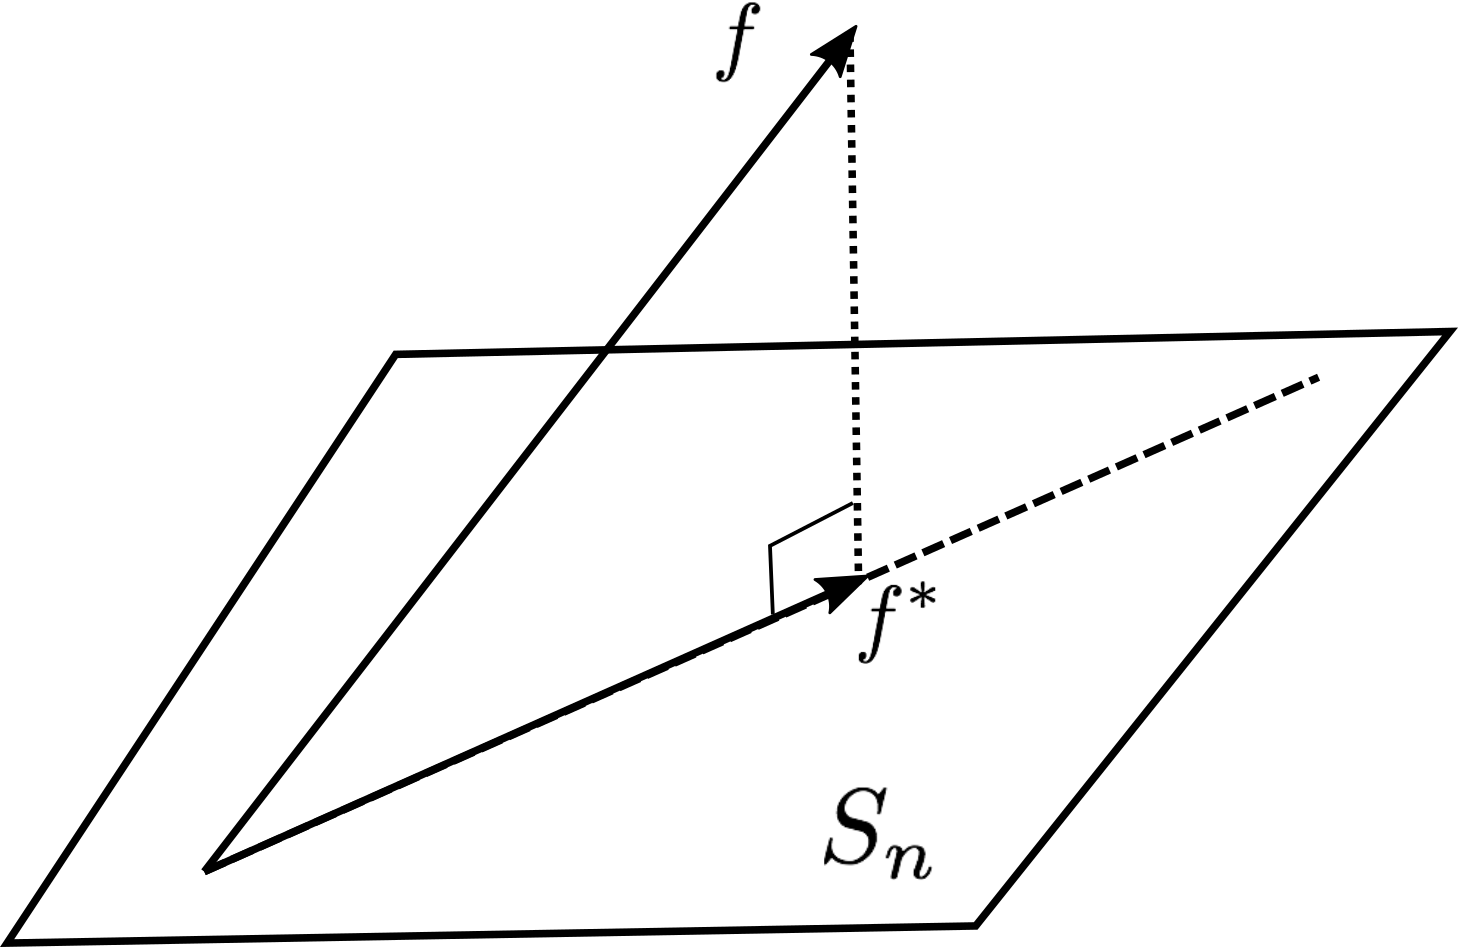
\includegraphics[height=8cm]{../image/least-square.png}
      \caption{最佳平方逼近几何含义}
      \label{fig: 最佳平方逼近几何含义}
    \end{figure}

\newpage
\subsection{正交多项式·绪论}
  \begin{defi}[正交]
    设函数$\f,\g\in\ms{C}[a, b]$,$\rho$为$[a, b]$上的权函数
    且满足
    \[
      (\f, \g) = \int_a^b\rho\f\g\rd x = 0,
    \]
    则称$\f$和$\g$在$[a, b]$上带权$\rho$\tbf{正交}. 若函数组
    $\{\varphi_k\}_{k=0}^\infty$满足
    \[
      (\varphi_i,\varphi_j) =
      \begin{cases}
        0,&\quad i\ne j \\
        A_k>0,& i=j
      \end{cases}
    \]
    则称$\{\varphi_k\}$为$[a, b]$上的带权$\rho$的\tbf{正交函数组}.
    若$A_k=1$,则称为\tbf{标准正交函数组}.
  \end{defi}

  \begin{defi}[正交多项式]
    设$\{\varphi_k\}_{k=0}^\infty$是首项系数$a_n\ne0$的$n$
    次多项式序列. 若它们正交,则称它们为\tbf{正交多项式序列}.
  \end{defi}

  \begin{alg}[Gram-Schmidt正交化]
    设$\{\varphi_k\}$是内积空间$V$的一组基,定义
    \[\begin{split}
      \psi_0 &= \varphi_0, \\
      \psi_{n} &= \varphi_n - \sum_{i=0}^{n-1}(\varphi_n, \psi_i)\eta_i
    \end{split}\]
    其中$\eta_i = \psi_i / \|\psi_i\|^2$. 则$\{\psi_k\}$为
    $V$的一组正交基.
  \end{alg}
  \remark
    要求$n$次正交多项式组,只需另$\varphi_k = x^k$,再进行
    Gram-Schmidt正交化即可.

  \begin{thm}
    设$\{\varphi_n\}_{n=0}^\infty$是一列正交多项式,
    根据正交性(从而线性无关)可以得到正交多项式的如下性质,
    \begin{enumerate}
      \item $P_n \subset \spn\{\varphi_0, \dots,\varphi_n\}$,
      \item 设$P\in P_{n-1}$,则$\varphi_n$与$P$正交.
    \end{enumerate}
  \end{thm}

  \begin{thm}
    设$\{\varphi_n\}_{n=0}^\infty$是$[a,b]$上带权$\rho$的
    正交多项式,则成立
    \[
      \varphi_{n+1} = (x-\alpha_n)\varphi_n - \beta_n\varphi_{n-1},
      \quad n = 0, 1,\dots,
    \]
    其中
    \[\begin{split}
      &\varphi_0 = 1,\quad \varphi_{-1} = 0,\\
      &\alpha_n = (x\varphi_n, \varphi_n) / (\varphi_n, \varphi_n),\\
      &\beta_n = (\varphi_n, \varphi_n) / (\varphi_{n-1}, \varphi_{n-1}).
    \end{split}\]
  \end{thm}
  \proof
    由于齐次性,不妨设$\varphi_n$首项系数为$1$. 所以成立
    \[
      \varphi_{n+1}-x\varphi_n = \sum_{k=0}^n\gamma_k\varphi_k,
    \]
    对于系数$\gamma_k$,成立
    \footnote{
      设$B$是内积空间$V$的一组正交基,则对于任意
      $x\in V$,成立
      \[
        x = \sum_{\beta\in B}\frac{(x,\beta)}{(\beta,\beta)}\beta
      \]
      另外,根据这里内积的定义,成立$(\varphi_i,\varphi_j)
      =(\varphi_i/x, x\varphi_j)$.
    }
    \[
      \gamma_k = \frac{(\varphi_{n+1}-x\varphi_n,\varphi_k)}
      {(\varphi_k, \varphi_k)}
      = \frac{(\varphi_{n+1},\varphi_k) - (\varphi_n, x\varphi_k)}{(\varphi_k,\varphi_k)}.
    \]
    由于$\{\varphi_n\}$正交,所以当$k<n-1$时,成立$\gamma_k=0$.
    所以有
    \[
      \varphi_{n+1} - x\varphi_n = \gamma_n\varphi_n + \gamma_{n-1}\varphi_{n-1}.
    \]
    再进行一些代换,即可以得到原递推式. $\blacksquare$

  \begin{thm}
    设$\{\varphi_n\}_{n=0}^\infty$为$[a, b]$上带权$\rho$的
    正交多项式,则$\varphi_n$在区间$(a, b)$上有$n$个不同的零点.
  \end{thm}
  \proof
    首先利用权函数的定义,证明零点不可能都是偶数重的. 再假设
    $x_1,\dots,x_l$是$\varphi_n$的奇数重零点,则
    \[
      \left(\varphi_n, (x-x_1)\cdots(x-x_l)) \right) \ne 0,
    \]
    再利用正交性可得$l=n$. $\blacksquare$

\newpage
\subsection{Legendre多项式}
  \begin{defi}[Legendre多项式]
    取区间$[-1, 1]$,$\rho(x)\equiv1$,称由$\{1,x,\dots,x^n,\dots\}$
    正交化而得的多项式为Legendre多项式. 其表达式为
    \[
      P_0(x) = 1,\quad
      P_n(x) = \frac{1}{2^nn!}\frac{\rd^n}{\rd x^n}(x^2-1)^n,
      \quad n=1,2,\dots
    \]
    首项系数为$1$的Legendre多项式为
    \[
      \widetilde{P}_n(x) = \frac{n!}{(2n)!}\frac{\rd^n}{\rd x^n}(x^2-1)^n.
    \]
  \end{defi}

  \begin{thm}[Legendre多项式的性质]
    Legendre多项式有如下性质,
    \begin{enumerate}
      \item 正交性:
      \[
        \int_{-1}^1 P_n(x)P_m(x)\rd x =
        \begin{cases}
            0, &\quad m\ne n, \\
            \dfrac{2}{2n+1},&\quad m = n.
        \end{cases}
      \]
      \item 奇偶性:
        \[P_n(x) = (-1)^nP_n(-x),\]
      \item 递推关系:
      \[
        (n+1)P_{n+1} = (2n+1)xP_n - nP_{n-1},\quad
        n = 1, 2,\dots
      \]
    \end{enumerate}
  \end{thm}
  \proof todo

  \begin{thm}[Legendre多项式的逼近性质]
    \label{thm: Legendre多项式的逼近性质}
    在区间$[-1, 1]$上,设$\widetilde{L}_n$是首项系数为$1$的
    Legendre多项式,则
    \[
      \|\widetilde{L}_n\|_2 = \min_{P\in P_n}\|P(x)\|_2.
    \]
  \end{thm}
  \remark
    应用方法和说明可以参考Chebyshev多项式的逼近性质.
    (\thmref{thm: Chebyshev多项式的逼近性质})

  \begin{lemma}[前$4$项Legendre多项式]
    \[\begin{split}
      P_0 &= 1,\\
      P_1 &= x,\\
      P_2 &= \frac{3}{2}x^2 - \frac{1}{2},\\
      P_3 &= \frac{5}{2}x^3 - \frac{3}{2}x
    \end{split}\]
  \end{lemma}

\newpage
\subsection{Chebyshev多项式}
  \begin{defi}[Chebyshev多项式]
    取区间$[-1, 1]$,$\rho(x)=(1-x^2)^{-1/2}$,称由$\{1,x,\dots,x^n,\dots\}$
    正交化而得的多项式为Chebyshev多项式. 其表达式为
    \[
      T_n(x) = \cos(n\arccos x),\quad|x|\le 1
    \]
  \end{defi}

  \begin{thm}[Chebyshev多项式的性质]
    Chebyshev多项式有如下性质,
    \begin{enumerate}
      \item 递推关系:
      \[\begin{split}
        &T_0(x) = 1, \quad T_1(x) = x,\\
        &T_{n+1}(x) = 2xT_n(x) - T_{n-1}(x),\quad n =1,2,\dots
      \end{split}\]
      \item 正交性:
      \[
        \int_{-1}^1\frac{T_n(x)T_m(x)}{\sqrt{1-x^2}} \rd x =
        \begin{cases}
          0, &\quad n\ne m,\\
          \pi/2, &\quad n = m \ne 0,\\
          \pi,&\quad n = m = 0.
        \end{cases}
      \]
      \item $T_{2k}(x)$只含$x$的偶次幂,$T_{2k+1}(x)$只含$x$的
      奇次幂.
      \item $T_n$在区间$[-1, 1]$上的$n$个零点为
      \[
        x_k = \cos\frac{2k-1}{2n}\pi,\quad k = 1,2,\dots,n.
      \]
      \item $T_n$的首项系数为$2^{n-1}$.
    \end{enumerate}
  \end{thm}

  \begin{thm}[Chebyshev多项式的逼近性质]
    \label{thm: Chebyshev多项式的逼近性质}
    在区间$[-1,1]$上,设$\widetilde{T}_n$是首项系数
    为$1$的Chebyshev多项式,则
    \[
      \|\widetilde{T}_n\|_\infty = \min_{P\in\widetilde{P}_n}
      \|P(x)\|_\infty = \frac{1}{2^{n-1}}.
    \]
  \end{thm}
  \remark
    这一定理意味着,取区间$[-1, 1]$,$n$次Chebyshev多项式是所有次数
    小于等于$n$的首项为$1$的多项式中,绝对值的最大值最小的一个. 从而,
    若想用$P_{n-1}$中的多项式来逼近$n$次多项式$\f$,只需找
    $\f^*\in P_{n-1}$,使得
    \[
      \f - \f^* = a_n \widetilde{T}_n.
    \]
    其中$a_n$为$\f$的$n$次项系数. 对于一般的在区间$[a, b]$上的情况,
    只需利用平移和伸缩映射到$[-1, 1]$上即可.

  \begin{thm}[Chebyshev零点插值]
    设插值节点$x_0,\dots,x_n$为Chebyshev多项式$T_{n+1}$的
    零点,被插值函数$\f\in\ms{C}^{n+1}[-1, 1]$,则多项式插值
    的余项$R_n$满足
    \[
      |R_n| \le \frac{1}{2^n(n+1)!}\|\f^{(n+1)}(x)\|_{\infty}.
    \]
  \end{thm}
  \proof
    由于插值点是Chebyshev多项式的零点,所以$\omega_{n+1}=
    \widetilde{T}_n$,所以根据\thmref{thm: Chebyshev多项式的逼近性质},成立
    \[
      \omega_{n+1} \le \frac{1}{2^n}.\quad\blacksquare
    \]
  \remark
    这一定理保证了使用Chebyshev多项式的零点插值,至少可以使得
    误差的最大值最小.


\newpage
\section{变分方法与数据拟合}
\subsection{绪论}
  若要求函数$\f(\mbf{x})$,$x\in\R^n$的最值点,根据
  Fermat引理,只需要求出所有成立$\nabla\f = 0$的点再
  逐一验证即可. 变分是这一思想的推广,它所处理的是过程的优化.
  下给出一个优化过程的例子,完整的解答见之后的章节. (todo: ref)

  \begin{exa}[最速降线]
    给定空中的一点$A=(0,0)$,地上一点$B=(x_1,y_1)$,求一条连接
    $A$和$B$的轨迹,使得假设在无阻力情况下,有小球沿轨道从$A$到$B$
    所需要的时间最短. \par
    假设轨道曲线充分光滑,则问题可以转换为,设滑行轨道$y\in\ms{C}^2$的方程为
    \[
      y=y(x), \quad y(0)=0,\quad y(x_1) = y_1.
    \]
    试确定曲线$y$使得时间$T(y)$最小. 根据机械能守恒,小球在$(*,-y)$处
    (见\figref{fig: 最速降线问题})的速度,为
    \[
      v = \sqrt{2gy},
    \]
    同时由速度的定义知
    \[
      v = \frac{\rd s}{\rd t} = \sqrt{1+y^{\pr2}(x)}\frac{\rd x}{\rd t},
    \]
    根据上两式,即有
    \[
      \sqrt{2gy}\rd t = \sqrt{1+y^{\pr2}(x)}\rd x \,\Rightarrow\,
      \rd t = \left( \frac{1+y^{\pr2}}{2gy} \right)^{1/2}\rd x
    \]
    设过程为$A\to B$,$0\to t_1$,$0\to x_1$,则
    \[
      T(y) = t_1 = \int_0^{x_1} \left( \frac{1+y^{\pr2}}{2gy} \right)^{1/2}\rd x,
    \]
    即为所要最小化的$T(y)$.
    \begin{figure}[htbp]
      \centering
      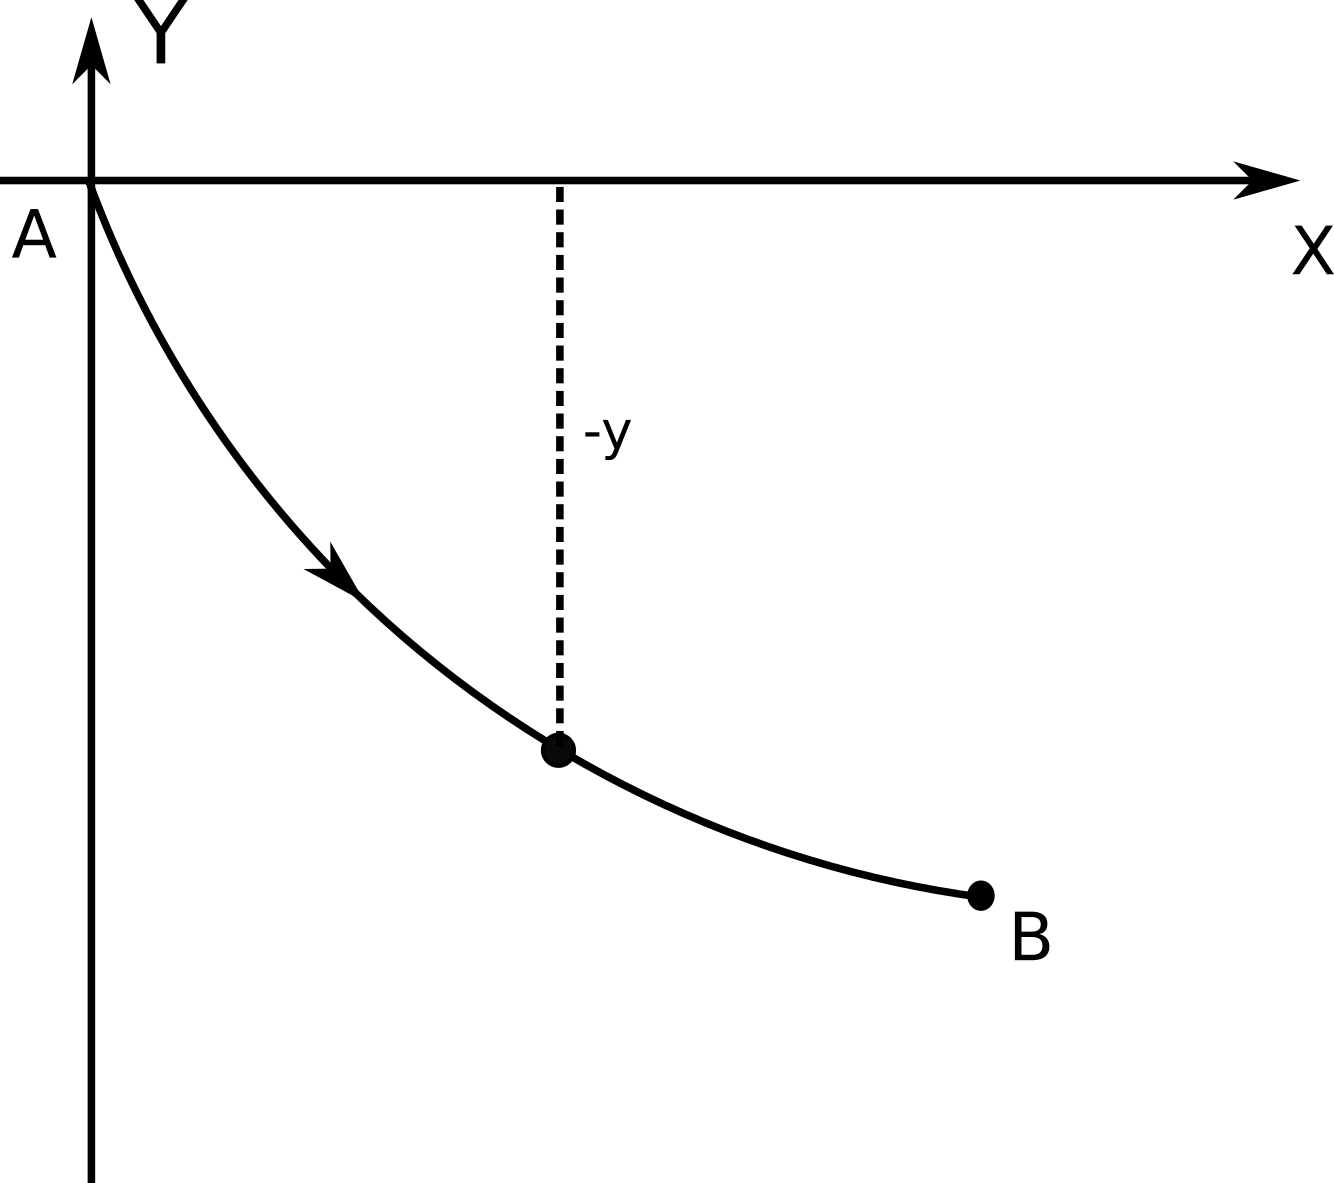
\includegraphics[height=5cm]{../image/brachistochrone.png}
      \caption{最速降线问题}
      \label{fig: 最速降线问题}
    \end{figure}
  \end{exa}

\newpage
\subsection{变分方法}
  \begin{defi}[过程优化]
    \label{def: 过程优化}
    过程的优化即求解
    \[
      \label{equ: 过程优化}
      y^* = \agm_{y\in K}J(y)
    \]
    的过程,其中函数集合
    \[
      K = \{y\in\ms{C}^2[x_0, x_1]\,:\, y(x_0)=y_0,\,y(x_1)=y_1\}.
    \]
  \end{defi}

  \begin{defi}
    \label{defi: K}
    定义函数集合
    \[\begin{split}
      K &= \{\f\in\ms{C}^2[x_0, x_1]\,:\,\f(x_0)=y_0,
      \f(x_1) = y_1\}, \\
      K_0 &=\{\f\in\ms{C}^2[x_0, x_1]\,:\,\f(x_0)=
      \f(x_1) = 0\}.
    \end{split}\]
    对于任意$\f_0\in K$,$\eta \in K_0$定义集合
    \[
      K(\f_0, \eta) = \{\f_0 + \vep\eta\,:\,\vep\in\R\}.
    \]
  \end{defi}

  \begin{defi}[泛函的方向导数]
    \label{def: 泛函的方向导数}
    记号同\defref{defi: K}. 定义泛函
    \[
      J(\f) = \int_a^bL(x, \f(x), \f\hp(x)) \rd x,\quad
      \f \in K.
    \]
    如果$\f^*$是函数$J(\f)$在集合$K$中的最小值点,即
    \[
      \f^* = \agm_{\f\in K}J(\f),
    \]
    则对于任意$\eta\in K_0$,$\f^*$也是$J(\f)$在集合$K(\f^*,\eta)$
    中的最小值点. 所以成立
    \[
      \f^* = \agm_{\vep\in\R}J(\f^* + \vep\eta).
    \]
    由于函数$J(\f^* + \vep\eta)$是关于实数$\vep$的一元函数,所以在
    它最小值点,即$\vep =0$处成立
    \begin{equation}
      \label{equ: 方向导数为零}
      \frac{\rd}{\rd\vep}J(\f^* + \vep\eta)\bigg|_{\vep =0}=0.
    \end{equation}
    称左侧为泛函$J$在$\f^*$处沿$\eta$方向的\tbf{变分}
    或\tbf{方向导数}. 即为$\delta J(\f^*, \eta)$\footnote{一般来讲,
    $\f^*$可以是集合中的任意一点. }.
  \end{defi}
  \remark
    这里采用的是分析学中一个常见思想,将一个在高维空间中的问题
    转化为一个低维空间中的问题. 一个更加简单的例子是,证明若
    $k$维欧式空间中的函数$\f$在凸集$K$中的各偏导数恒为零,则
    它在$K$中为常量. 一个证法是取定$K$中任意一点(向量)$\mbf{x}_0$,
    则对于任意$\mbf{x}\in K$,则对于任意直线段$xx_0$,有方程
    \[
      y = \mbf{x_0}t + \mbf{x}(1-t).
    \]
    上式是一个一元实函数,对它求导并利用一元函数微分学中的知识,可以
    知道在这条直线段上$\f$的函数值不变. 由于$\mbf{x}_0$和$\mbf{x}$
    的选取是任意的,所以在$K$上$\f$的值不变. \par
    在这里采用的是同样的思想,只是把欧式空间换成了一个函数集合而已.

  \begin{lemma}[变分引理 I]
    \label{lemma: 变分引理}
    设$\f\in\ms{C}[a,b]$,且对任意满足$\g(a)=\g(b)=0$的
    $\g\in\ms{C}^2[a,b]$,有
    \[
      \int_{a}^{b}\f\g \rd x =0,
    \]
    则在$[a,b]$上成立$\f\equiv 0$.
  \end{lemma}

  \begin{lemma}[变分引理 II]
    设$\f\in\ms{C}[a, b]$,且对于任意满足$\eta(a) = \eta(b) = 0$的
    $\eta\in\ms{C}^1(a, b)$都成立
    \[
      \int_a^b\f\eta\hp\rd x = 0,
    \]
    则在$[a, b]$上成立$\f\equiv \text{Const}$.
  \end{lemma}

  \begin{thm}[Euler-Lagrange方程]
    \label{thm: Euler-Lagrange方程}
    记号同\defref{def: 泛函的方向导数}. 泛函$J(\f)$在极值点满足
    Euler-Lagrange方程
    \begin{equation}
      \label{equ: Euler-Lagrange方程}
      \frac{\partial L}{\partial\f} - \frac{\rd}{\rd x}\frac{\partial L}{\partial\f\hp} = 0.
    \end{equation}
  \end{thm}
  \proof
    假设满足求导积分换序的条件,则泛函$J(\f)$在
    $\f_*+\vep\eta$处沿$\eta$方向的方向导数为
    \footnote{为了记号的清晰,这里用$\f_*$替代之前的$\f^*$.
    并且这里关于偏导数的记号,应理解为关于分母所表示的那一分量的偏导数. }
    \[\begin{split}
      \frac{\rd}{\rd\vep}J(\f_*+\vep\eta) &=
      \frac{\rd}{\rd\vep}\int_{x_0}^{x_1}L(x,\f_*+\vep\eta,\f_*\hp+\vep\eta\hp)\rd x\\
      &= \int_{x_0}^{x_1} \frac{\partial L}{\partial (\f_*+\vep\eta)}\eta
      +\frac{\partial L}{\partial (\f_*\hp+\vep\eta\hp)}\eta\hp\,\rd x.
    \end{split}\]
    代入$\vep=0$,即得$J$在最小值点$\f_*$处的方向导数,为
    \[\begin{split}
      \frac{\rd}{\rd\vep}J(\f_*) &=
      \int_{x_0}^{x_1} \frac{\partial L}{\partial \f}\eta
      +\frac{\partial L}{\partial \f\hp}\eta\hp\,\rd x \\
      &= \int_{x_0}^{x_1} \frac{\partial L}{\partial\f}\eta\rd x
      + \frac{\partial L}{\partial\f\hp}\eta\bigg|_{x_0}^{x_1}
      - \int_{x_0}^{x_1}\eta\frac{\rd}{\rd x}\frac{\partial L}{\partial \f\hp}\rd x\\
      &= \int_{x_0}^{x_1} \eta\left( \frac{\partial L}{\partial\f}
      - \frac{\rd}{\rd x}\frac{\partial L}{\partial\f\hp} \right) \rd x = 0.
    \end{split}\]
    注意由于$\eta\in K_0$,即有$\eta(x_0) = \eta(x_1) = 0$.
    由于$\eta$的选取是任意的,所以根据\lemmaref{lemma: 变分引理},式子
    \equref{equ: Euler-Lagrange方程}成立. $\blacksquare$
  \remark
    对于$L = L(\f,\f\hp)$,即$L$不显含$x$的情况,
    \equref{equ: Euler-Lagrange方程}是可以精确求解的.

  \begin{thm}[守恒律定理]
    \label{thm: 守恒律定理}
    设$L = L(\f,\f\hp)$,则沿着\equref{equ: 过程优化}的解曲线
    $y^* = \f^*(x)$,成立
    \[
      H = \f\hp\frac{\partial L}{\partial\f\hp} - L = \text{Const}.
    \]
  \end{thm}
  \proof
    \[\begin{split}
     \frac{\rd H}{\rd x} &= \frac{\rd}{\rd x}
     \left( \f\hp\frac{\partial L}{\partial\f\hp}-L(\f,\f\hp) \right)\\
     &= \f^{\pr\pr}\frac{\partial L}{\partial\f\hp}
     + \f\hp\frac{\rd}{\rd x}\frac{\partial L}{\partial\f\hp} -
     \frac{\partial L}{\rd\f}\f\hp -
     \frac{\partial L}{\rd\f\hp}\f^{\pr\pr}.
    \end{split}\]
    根据\thmref{thm: Euler-Lagrange方程},$\rd H /\rd x =0$,所以
    命题成立. $\blacksquare$

  % \begin{exa}[最速降线的求解]
  %   根据之前的讨论,即求解
  %   \[
  %     \f_* = \agm_{\f\in K} T(\f) = \int_{0}^{x_1}
  %     \left( \frac{1+\f\hp}{2g\f} \right)^{1/2}\rd x.
  %   \]
  %   根据\thmref{thm: 守恒律定理},成立
  %   \[
  %
  %   \]
  % \end{exa}

\newpage
\subsection{曲线拟合的正则化方法}
  \begin{defi}[Tikhonov正则化]
    \label{def: Tikhonov正则化}
    对于给定的数据$Y$,定义数据拟合项为$J_1(\f)$,用于表示拟合结果
    相较于原数据的接近程度,同时要求拟合的结果尽可能满足对于结果的
    要求,用$J_2(\f)$来描述$\f$满足要求的程度,则求解拟合结果的
    过程即为求解
    \[
      \f_* = \agm_{\f\in K}(J_1(\f) + \alpha J_2(\f)).
    \]
    其中$\alpha$为\tbf{正则化参数},用于表示拟合的过程中,应更接近
    原数据或是更满足拟合要求. 若取$\alpha=0$,即为插值.
  \end{defi}

  \begin{prob}
    给定函数$y$在样本点$0=x_0 < x_1 < \cdots < x_n = 1$处的
    近似值$\tilde{y}_i$,误差满足
    \[
      |\tilde{y}_i - y(x_i)| \le \delta,
    \]
    试重构$y$的近似函数$\f_*$.\par
    按照\defref{def: Tikhonov正则化}的思想,定义
    \[\begin{split}
      J_1(\f) &= \sum_{i=1}^{n-1}\frac{h_i+h_{i+1}}{2}
      \left( \tilde{y}_i - \f(x_i) \right)^2 \\
      J_2(\f) &= \int_0^1 (\f^{\pr\pr})^2\rd x
    \end{split}\]
    其中
    \[\begin{split}
      h_i &= x_i - x_{i-1},\quad i = 1,2,\dots,n\\
      h &= \max_{1\le i\le n}h_i
    \end{split}\]
    则问题转换为求解
    \begin{equation}
      \label{equ: 正则化曲线拟合}
      \f_* = \agm_{\f\in K}\left( J_1(\f) + \alpha J_2(\f) \right).
    \end{equation}
  \end{prob}
  \remark
    不失一般性的,可以设$\tilde{y}_0 = \f(x_0)$且$\tilde{y}_n=\f(x_n)$.
    否则只需要用
    \[
      Y(x) = y(x)+\tilde{y}_0-y(0)+(\tilde{y}_n-y(1)+y(0)-\tilde{y}_n)x
    \]
    来替代$y$即可. 可以证明
    \begin{enumerate}
      \item $Y(0) = \tilde{y}_0$且$Y(1) = \tilde{y}_n$,
      \item $|\tilde{y}_i - Y(x_i)| \le 4\delta$.
    \end{enumerate}

  \begin{thm}
    对于任意$\alpha>0$,\equref{equ: 正则化曲线拟合}的解为三次样条函数.
  \end{thm}
  \proof
    设$\f_*$为式\equref{equ: 正则化曲线拟合}的解. \par
    对于任意$\eta\in K_0$,$\vep\in R$,
    \[
      J(\f_*+\vep\eta) = \sum_{i=1}^{n-1}\frac{h_i + h_{i+1}}{2}
      [\tilde{y}_i - f_*(x_i) - \vep\eta(x_i)]^2 + \alpha
      \int_0^1(\f_*^{\pr\pr} + \vep\eta^{\pr\pr})^2\,\rd x.
    \]
    求它关于$\vep$的导数,成立
    \[
      \frac{\rd}{\rd\vep}J(\f_*+\vep\eta) =
      -2\sum_{i=1}^{n-1}\frac{h_i+h_{i+1}}{2}[\tilde{y}_i-\f_*(x_i)-\vep\eta(x_i)]\eta(x_i)
      +2\alpha\int_0^1 (\f_*^{\pr\pr}+\vep\eta^{\pr\pr})\eta^{\pr\pr} \,\rd x.
    \]
    根据\defref{def: 泛函的方向导数}中的\equref{equ: 方向导数为零},上式在$\vep=0$时
    值为零,即
    \begin{equation}
      \label{equ: 正则化证明1}
      \frac{\rd}{\rd\vep}J(\f_*+\vep\eta)\bigg|_{\vep=0} =
      -2\sum_{i=1}^{n-1}\frac{h_i+h_{i+1}}{2}[\tilde{y}_i-\f_*(x_i)]\eta(x_i)
      +2\alpha\int_0^1\f_*^{\pr\pr}\eta^{\pr\pr}\,\rd x = 0.
    \end{equation}
    接下来分两步构造出$\f_*$.\\
  \tbf{Step 1. }
    由于$\eta$的选取是任意的,所以我们选择恰当的$\eta\in\ms{C}^\infty(x_i,x_{i+1})$,
    使得成立
    \[
      \eta(x_i) = 0,\quad i = 1,2,\dots,n-1
    \]
    所以根据\equref{equ: 正则化证明1},成立
    \[
      \int_{x_i}^{x_{i+1}}\f_*^{\pr\pr}\eta^{\pr\pr} = 0.
    \]
    对于上式进行两次分部积分,得到
    \[
      0 = \f_*^{\pr\pr}\eta\hp\bigg|_{x_i}^{x_{i+1}} -
      \f_*^{(3)}\eta\bigg|_{x_i}^{x_{i+1}} +
      \int_{x_i}^{x_{i+1}}\f_*^{(4)}\eta\rd x.
    \]
    同样因为$\eta$的选取是任意的,所以可以在原来的基础上,选取$\eta$使得成立
    \[
      \eta(x_i) = \eta\hp(x_i) = 0,\quad i = 1,2,\dots,n-1
    \]
    所以有
    \[
      \int_{x_i}^{x_{i+1}}\f_*^{(4)}\eta\rd x = 0.
    \]
    根据变分引理,即成立
    \begin{equation}
      \label{equ: 正则化证明2}
      \f_*^{(4)}(x) = 0\quad\Rightarrow\quad \f\in P_3,\quad x\in(x_i,x_{i+1}).
    \end{equation}
  \tbf{Step 2. }
    取满足$\eta(0)=\eta(1)=0$的$\eta\in\ms{C}^\infty[0, 1]$,分部积分得
    (注意$\f_*^{(4)} = 0$)
    \[\begin{split}
      \int_0^1 \f_*^{\pr\pr}\eta^{\pr\pr}\rd x =&
      \sum_{i=1}^{n-1}
      \left(
        -\f_*^{(3)}\eta\bigg|_{x_i-1}^{x_i}
        +\f_*^{\pr\pr}\eta\hp\bigg|_{x_i-1}^{x_i}
      \right) \\
      =& \sum_{i=1}^{n-1}
      ( \f_*^{(3)}(x_i+) - \f_*^{(3)}(x_i-))\eta(x_i) +
      \sum_{i=1}^{n-1} ( \f_*^{\pr\pr}(x_i+) - \f_*^{\pr\pr}(x_i-))\eta\hp(x_i)\\
      & + \f_*^{\pr\pr}(1)\eta\hp(1) - \f_*^{\pr\pr}(0)\eta\hp(0)
    \end{split}\]
    将结果带入\equref{equ: 正则化证明1},即
    \begin{equation}\begin{split}
      \label{equ: 正则化证明3}
      0 =&
      \f_*^{\pr\pr}(1)\eta\hp(1) - \f_*^{\pr\pr}(0)\eta\hp(0)\\
      &+\sum_{i=1}^{n-1} \left(
        -\frac{h_i+h_{i+1}}{2}[\tilde{y}_i - \f_*(x_i)]
        + \alpha(\f_*^{(3)}(x_i+) - \f_*^{(3)}(x_i-))
      \right)\eta(x_i) \\
      &+\alpha\sum_{i=1}^{n-1} ( \f_*^{\pr\pr}(x_i+) - \f_*^{\pr\pr}(x_i-))\eta\hp(x_i)
    \end{split}\end{equation}
    由于$\eta$的选取是任意的,即意味着$\eta(x_i)$,$(i=1,2,\dots,n-1)$和
    $\eta\hp(x_i)$,$(i=0,1,\dots,n)$的选取是任意的,所以需要选取适当的$\f$才可以使得
    \equref{equ: 正则化证明3}中的每一项都恒为零. 为使第$1$、$3$项为零,需要满足
    \[\begin{split}
      & \f_*^{\pr\pr}(1) = \f^{\pr\pr}(0) = 0,\\
      & \f_*^{\pr\pr}(x_i+) = \f_*^{\pr\pr}(x_i-).
    \end{split}\]
    同样的,根据不同的$\alpha$,选取恰当的$\f(x_i)$或
    $\f^{(3)}(x_i)$使得第二项为零.
    综合上式以及\equref{equ: 正则化证明2},可知$\f_*$为三次样条函数,
    且当$\alpha=0$时为样条插值函数. $\blacksquare$


\newpage
\section{数值积分与数值微分}
\subsection{绪论}
  \begin{thm}[N-L公式]
    设$\f$和$F$定义在$[a, b]$上,$F \in \ms{C}[a, b]$且在
    $(a, b)$上成立$F\hp=\f$,则
    \[
      \int_a^b \f(x)\rd x = F(b) - F(a).
    \]
  \end{thm}
  \remark
    N-L公式是求解积分的基本方法. 但是$F(x)$通常是难以求解的,
    所以需要数值方法.

  \begin{thm}[积分第一中值定理]
    \label{thm: 积分第一中值定理}
    设$\f\in\ms{C}[a, b]$,$\g\in\ms{R}[a, b]$且不变号,
    则存在$\xi\in[a, b]$,成立
    \[
      \int_a^b\f(x)\g(x)\rd x = \f(\xi)\int_a^b\g(x)\rd x.
    \]
  \end{thm}
  \proof
    不妨设$\g(x)\ge 0$. 若$\g(x)\equiv 0$,则结论是显然的.
    考虑$\g$不恒为零的情况. 由于$\f\in\ms{C}$,所以$\f$在$[a,b]$
    上可以取到最小值$m$和最大值$M$,则成立
    \[\begin{split}
      & m\g(x) \le \f(x)\g(x) \le M\g(x) \\
      \Rightarrow \quad &
      m\int_a^b\g(x)\rd x \le \int_a^b\f(x)\g(x)\rd x
      \le M\int_a^b\g(x)\rd x \\
      \Rightarrow \quad &
      m \le \frac{\int_a^b\f(x)\g(x)\rd x}{\int_a^b\g(x)\rd x}
      \le M
    \end{split}\]
    由于连续函数有介质性,所以存在$\xi\in[a, b]$成立
    \[
      \f(\xi) = \frac{\int_a^b\f(x)\g(x)\rd x}{\int_a^b\g(x)\rd x}.
    \]
    即成立
    \[
      \int_a^b\f(x)\g(x)\rd x = \f(\xi)\int_a^b\g(x)\rd x.
      \quad\blacksquare
    \]
  \remark
    注意,定理要求$\f\in\ms{C}[a, b]$,这在很多情况下是难以
    满足的. 但是有些时候可以利用证明中的思路,在$\f$不连续的情况
    下得出同样的结论.

  \begin{pos}
    \label{pos: 积分第一中值定理2}
    设$\f\in\ms{C}[a, b]$,$\g\in\ms{R}[a, b]$且不变号,
    $\psi:[a, b]\to[a, b]$,则存在$\xi\in[a, b]$,使得
    \[
      \int_a^b\f(\psi(x))\g(x)\rd x =
      \f(\xi)\int_a^b\g(x)\rd x.
    \]
  \end{pos}
  \remark
    证明同\thmref{thm: 积分第一中值定理}是几乎一样的。

  \begin{pos}[中矩形公式]
    \label{pos: 中矩形公式}
    设$\f$足够光滑,则
    \[
      \int_a^b\f\rd \approx \f\left(\frac{a+b}{2}\right)(b-a).
    \]
    且存在$\xi\in[a, b]$,其误差$R(\f)=\lhs-\rhs$满足
    \[
      R(\f) = \frac{1}{24}(b-a)^3\f^{\pr\pr}(\xi).
    \]
  \end{pos}
  \proof
    \[\begin{split}
      R(\f) &= \int_a^b\f(x)\rd x - (b-a)\f\left( \frac{a+b}{2} \right) = \int_a^b \left[
        \f(x) - \f\left(\frac{a+b}{2}\right)
      \right]\rd x
    \end{split}\]
    在$x = (a+b)/2$处带Lagrange余项Taylor展开,有
    \[\begin{split}
      R(\f) &= \int_a^b\left[ \f\hp\left(\frac{a+b}{2}\right)\left(x - \frac{a+b}{2}\right)
       + \frac{1}{2}\f^{\pr\pr}(\xi(x))\left(x - \frac{a+b}{2}\right)^2\right]\rd x \\
       &= \frac{1}{2}\int_a^b\f^{\pr\pr}(\xi(x))\left(x - \frac{a+b}{2}\right)^2\rd x
    \end{split}\]
    由于$\xi(x)$的连续性是无法保证的,所以无法直接使用积分中值定理. 但是可以
    根据\posref{pos: 积分第一中值定理2}得,存在$\zeta\in[a, b]$,成立
    \[
      R(\f) = \frac{1}{2}\f^{\pr\pr}(\zeta)\int_a^b\left( x-\frac{a+b}{2} \right)^2\rd x
      = \frac{1}{24}(b-a)^3\f^{\pr\pr}(\zeta).\quad\blacksquare
    \]

  \begin{pos}[梯形公式]
    设$\f$足够光滑,则
    \[
      \int_a^b\f(x)\rd x \approx \frac{\f(a)+\f(b)}{2}(b-a)
    \]
    且存在$\xi\in[a, b]$,其误差$R(\f)=\lhs-\rhs$满足
    \[
      R(\f) = -\frac{1}{12}(b-a)^3\f^{\pr\pr}(\xi).
    \]
  \end{pos}
  \remark
    证明同\posref{pos: 中矩形公式}的证明是相似的. 实际上梯形公式
    可以理解为对原有的函数进行线性插值,并用插值结果的积分来近似原函数
    的积分. 按照这一思路推广,即发现可以用插值多项式的积分来近似原来
    函数的积分.

  \begin{pos}[Simpson公式]
    设$\f$足够光滑,则
    \[
      \int_a^b\f(x)\rd x \approx \frac{b-a}{6}
      \left[ \f(a) + 4\f\left(\frac{a+b}{2}\right)+\f(b) \right].
    \]
    存在$\xi\in[a,b]$,其误差$R(\f)=\lhs-\rhs$满足
    \[
      R(\f) = -\frac{(b-a)^5}{2880}\f^{(4)}(\xi).
    \]
  \end{pos}
  \remark
    实际上这是以$a$,$b$,$(a+b)/2$作插值节点作二次多项式插值后
    的函数积分后的结果. 但是若按照之前的思路证明,会发现$g(x)
    =(x-a)(x-(a+b)/2)(x-b)$在$[a, b]$上是不保号的,所以不能直接
    沿用之前的做法. 为了让它保号,我们可以采用Hermite插值,具体证
    法见下. 另外,有人或许会尝试把它拆分到两个区间上,让$\g$分别保号,
    但这样的做法一般来说是错误的,问题出现在最后一步合并两个区间结果的
    时候,权重有可能会出现负值.
  \proof
    设Hermite插值多项式$H\in P_3$满足$H(a) = \f(a)$,$H(b) = \f(b)$,
    $H((a+b)/2)) = \f((a+b)/2)$,$H\hp((a+b)/2) = \f\hp((a+b)/2)$.
    则存在$\xi\in[a, b]$,使其误差满足
    \[
      \f(x) - H(x) = \frac{\f^{(4)}(\xi)}{4!}(x-a)\left(\frac{a+b}{2}\right)^2(x-b).
    \]
    它在$[a,b]$上是保号的. 对$H(x)$积分即可得$\rhs$. 剩下的内容和之前
    的证明是相同的. $\blacksquare$
  \remark
    根据余项公式可以发现,Simpson公式对于$\f\in P_3$都是精确
    成立的,基于此思想,定义代数精度.

  \begin{defi}[代数精度]
    记\footnote{在以后若不特殊说明,此记号都表示在$[a, b]$上的积分. }
    \[
      I(\f) = \int_a^b\f(x)\rd x.
    \]
    若数值积分公式
    \[
      I(\f) \approx Q(\f)
    \]
    在$\f\in P_n$时精确成立,在$\f\in P_{n+1}$时不精确成立,则称该
    求积公式有$n$阶代数精度.
  \end{defi}
  \remark
    代数精度是求积公式精确程度的一个度量,通常希望求积公式有更高的
    代数精度.

  \begin{defi}[机械求积公式]
    \label{defi: 机械求积公式}
    称求积公式为机械求积公式,若它满足
    \[
      I(\f) = \sum_{k=0}^nA_k\f(x_k).
    \]
    称$x_k\in[a, b]$为求积节点,称$A_k$为求积系数,它的选取与被积函数
    无关,至于求积节点有关.
  \end{defi}
  \remark
    可以发现这一节中出现的求积公式都是机械求积公式,但它们的误差各不相同.
    我们希望可以通过恰当地选取求积节点$x_k$和求积系数$A_k$,使得求积公式
    的代数精度尽可能高. \par
    若我们希望机械求积公式有$m$次代数精度,即意味着对于$1,x,\dots,x^m$
    的积分都是精确成立的,即成立非线性方程组
    \[\begin{split}
      &\sum A_k = b-a,\\
      &\sum A_kx_k = \frac{1}{2}(b^2-a^2),\\
      &\cdots\cdots \\
      &\sum A_kx_k^m = \frac{1}{m+1}(b^{m+1}-a^{m+1}).
    \end{split}\]
    这一方程组求解通常是困难的.

  \begin{defi}[插值求积公式]
    给定节点$a\le x_0 < \cdots < x_n \le n$处的函数值$\f(x_i)$,
    构造$n$次Lagrange多项式,则有
    \[
      I(\f) \approx \sum_{k=0}^n\left( \int_a^bl_k\rd x \right)\f(x_k).
    \]
    $l_k$的定义见\thmref{thm: Lagrange插值法}. 其误差满足
    \[
      R(\f) = \frac{\f^{(n+1)}(\xi)}{(n+1)!}\omega_{n+1}(x)
    \]
  \end{defi}

  \begin{defi}[收敛]
    对于求积公式
    \[
      \sum_{k=0}^n A_k\f(x_k) \approx \int_a^b\f\rd x
    \]
    记$h = \max\{x_i-x_{i-1}\}$,若当$h\to 0$时,$\lhs\to\rhs$,
    则称求积公式是收敛的.
  \end{defi}

  \begin{defi}[稳定]
    设$\tilde{\f}_k$是$\f(x_k)$的近似值. 对于任意的$\vep>0$,
    如果存在$\delta>0$,只需$|\tilde{\f}_k - \f(x_k)|<\delta$,
    就成立
    \[
      \left| Q(\f) - Q(\tilde{\f}) \right| =
      \left| \sum_{k=0}^nA_k(\f(x_k) - \tilde{\f}_k) \right| < \vep,
    \]
    则称求积公式是稳定的.
  \end{defi}
  \remark
    一个求积公式稳定,意味着测量误差并不会随着计算而扩大.

  \begin{thm}[稳定性条件]
    如果机械求积公式的系数$A_k>0$,则该求积公式是稳定的.
  \end{thm}

\subsection{Newton-Cotes公式}
  \begin{thm}[Newton-Cotes公式]
    将积分区间$[a, b]$ $n$等分,步长$h=\frac{b-a}{n}$,构造插值型
    求积公式,即
    \[
      Q(\f) = (b-a)\sum_{k=0}^n C_k^{(n)}\f(x_k)
    \]
    称为Newton-Cotes公式,其中$C_k^{(n)}$称为Cotes系数,为
    \[
      C_k^{(n)} = \frac{h}{b-a}\int_0^n \prod_{j=0,\,j\ne k}^n\frac{t-j}{k-j}\rd t
       = \frac{(-1)^{n-k}}{nk!(n-k)!}\int_0^n\prod_{j=0,\,j\ne k}^n(t-j)\rd t
    \]
  \end{thm}
  \remark
    当$n\ge 8$的时候,Cotes系数出现负值,意味着测量误差会随着计算而增大,所以
    $n\ge 8$的Newton-Cotes公式是不用的.

  \begin{thm}[插值型求积公式的代数精度]
    形如
    \[
      Q(\f) = \sum_{k=0}^nA_k\f(x_k)
    \]
    的求积公式有$n$次或以上代数精度的充要条件为,它是插值型的.
  \end{thm}
  \proof
    充分性是显然的. 对于必要性,用$Q(\f)$计算$l_k$来得到$A_k$,即
    \[
      \int_a^bl_k(x)\rd x = \sum_{j=0}^nA_jl_k(x_j) \quad\Rightarrow\quad
      A_k = \int_a^bl_k(x)\rd x.\quad\blacksquare
    \]

  \begin{thm}[偶阶求积公式的代数精度]
    当$n$为偶数时,$n$阶插值型求积公式至少有$n+1$次代数精度.
  \end{thm}

\subsection{复合求积公式}
  即对原积分区间$n$等分,使得每一段长度$h<1$,之后在每一段上
  分别求积。

  \begin{thm}[复合梯形公式余项]
    \[
      T_n(\f) = \frac{h}{2}[\f(a) + 2\sum_{k=1}^{n-1}\f(x_k) + \f(b)]
    \]
    其余项为
    \[
      R_n(\f) = -\frac{b-a}{12}h^2\f^{\pr\pr}(\eta),\quad
      \eta\in[a, b]
    \]
  \end{thm}

  \begin{thm}[复合Simpson公式]
    \[
      S_n = \frac{h}{6}[\f(a) + 4\sum_{k=0}^{n-1}\f(x_{k+1/2})
      + 2\sum_{k=1}^{n-1}\f(x_k) + \f(b)]
    \]
    其余项为
    \[
      R_n(\f) = -\frac{b-a}{180}\left(\frac{h}{2}\right)^4\f^{(4)}(\eta),
      \quad\eta\in[a, b]
    \]
  \end{thm}

\subsection{Gauss求积公式}
  \begin{pos}[求积公式代数精度上限]
    形如下式的求积公式的代数精度至多为$2n+1$.
    \[
      \int_a^b\f(x)\rd x\approx \sum_{k=0}^nA_k\f(x_k).
    \]
  \end{pos}
  \remark
    根据本节之后的构造,可以发现这个上限是取得到的.

  \begin{defi}[Gauss求积公式]
    设
    \begin{equation}
      \label{equ: 带权求积公式}
      I(\f) = \int_a^b\f(x)\rho(x)\rd x \approx \sum_{k=0}^nA_k\f(x_k) = Q(\f).
    \end{equation}
    若\equref{equ: 带权求积公式}有$2n+1$次代数精度,则称其节点$x_k$为Gauss点,
    称该公式为Gauss型求积公式.
  \end{defi}
  \remark
    若要解权函数对应的Gauss求积公式,则只需要取$\f(x) = x^k$,$k=
    0,1,\dots, 2n+1$,解对应的方程组即可. 但由于它是关于$x_k$和
    $A_k$非线性的方程组,所以需要先确定$x_k$,得到关于$A_k$的线性
    方程组.

  \begin{thm}
    节点为$a \le x_0 < \cdots < x_n = b$的带权机械求积公式$Q(\f)$有
    $n+k$($0\le k\le n+1$)次代数精度的充要条件为:
    \begin{enumerate}
      \item $Q(\f)$为插值型求积公式,
      \item 对任意$p\in P_{k-1}$,成立
      \[
        \int_a^b\rho(x)p(x)\omega_{n+1}(x)\rd x = 0
      \]
    \end{enumerate}
  \end{thm}
  \proof
    todo

  \begin{cor}
    \equref{equ: 带权求积公式}有$2n+1$次代数精度,当且仅当
    节点$\{x_i\}$是$n+1$次正交多项式的根.
  \end{cor}
  \remark
    若积分区间为$[a, b]$,一般会先变换到$[-1, 1]$上. 之后的讨论
    中的区间都选取$[-1, 1]$.

  \begin{pos}
    Gauss求积公式的系数全是正的,从而它是稳定的.
  \end{pos}

  \begin{thm}
      Gauss求积公式是收敛的,即
      \[
        \lim_{n\to\infty}\sum_{k=0}^nA_k\f(x_k)
        = \int_a^b\rho\f\rd x.
      \]
  \end{thm}

\subsection{Romberg求积公式}
  \paragraph{动机}
    在利用复合求积公式的时候,如果需要增加精度,则需要再二分一遍区间.
    即增加了节点$x_{k+\frac{1}{2}} = \frac{1}{2}(x_k + x_{k+1})$.
    如果每次增加节点后都需要按照求积公式重新计算,则显然计算量过大并且浪费
    了先前计算好的结果,所以希望可以充分地利用先前的计算结果来简化计算.

  \begin{alg}[Richardson外推方法]
    \label{alg: Richardson外推方法}
    设$Q$为需要计算的值的精确结果,$Q_1(h)$是通过某一算法计算得
    的$Q$的近似,若误差满足
    \begin{equation}
      \label{equ: Q-Q(h)}
      Q-Q_1(h) = c_1h^{p_1} + c_2h^{p_2} + \cdots = o(h^{p_1-1})
    \end{equation}
    其中$0<p_1<p_2<\cdots$与$h$无关. 则令
    \[
      Q_{k+1}(h) = \frac{Q_k(h/2) - 2^{-p_k}Q_k(h)}{1-2^{-p_k}}.
    \]
    其误差满足
    \[
      Q-Q_{k+1}(h) = c_2^*h^{p_2} + c_3^*h^{p_3} + \cdots = o(h^{p_2-1})
    \]
  \end{alg}
  \remark
    Richardson外推方法意味着如果有二分前的结果$Q(h)$
    和二分后的结果$Q(h/2)$,那么可以通过这两个结果做一次外推
    从而得到更高的精度. 并且二分了多少次,就可以外推多少次.
  \proof
    根据\equref{equ: Q-Q(h)},成立
    \[\begin{split}
      Q - Q(h/2) &= c_1\left(\frac{h}{2}\right)^{p_1} + c_2\left(\frac{h}{2}\right)^{p_2} + \cdots\\
      2^{-p_1}(Q-Q(h)) &= c_1\left(\frac{h}{2}\right)^{p_1} + c_22^{-p_1}h^{p_2} + \cdots\\
    \end{split}\]
    将上述两式相减,即成立
    \[\begin{split}
      &Q-Q(h/2) - 2^{-p_1}(Q-Q(h)) = c_2^*h^{p_2} + c_3^*h^{p_3} + \cdots\\
      \Rightarrow\quad&
      Q_2(h) = \frac{Q(h/2) - 2^{-p_1}Q(h)}{1-2^{-p_1}}\quad\blacksquare
    \end{split}\]

  \begin{pos}
    复合梯形公式外推一次即得Simpson公式,
  \end{pos}

  \begin{pos}[复合梯形公式余项]
    \label{pos: 复合梯形公式余项}
    对于$[a, b]$进行$n$等分,令$h = (b-a)/n$,考虑复合梯形求积公式
    \[
      T(h) = h\left[ \frac{\f(x_0)}{2} + \f(x_1)
      +\cdots + \f(x_{n-1}) + \frac{\f(x_n)}{2} \right].
    \]
    存在与$h$无关的$a_i$,成立
    \[
      T(h) = \int_a^b\f\rd x + \sum_{k=1}^\infty a_{2k}h^{2k}.
    \]
  \end{pos}

  \begin{alg}[Romberg算法]
    记$n$次二等分第$m$次外推后的结果是$R(n, m)$,记
    $h_n = \frac{1}{2^n}(b-a)$,则
    \[\begin{split}
      R(0, 0) &= h_1(\f(a) + \f(b)) \\
      R(n, 0) &= \frac{1}{2}R(n-1, 0)
      + h_n\sum_{k=1}^{2^{n-1}}\f(a+(2k-1)h_n) \\
      R(n, m) &= \frac{1}{4^m-1}(
        4^mR(n,m-1) - R(n-1,m-1)
      )
    \end{split}\]
    其余项是$O(h_n^{2(m-1)})$的.
  \end{alg}
  \remark
    $R(n, 0)$是二等分$n$次后的复合梯形公式的结果,它可以通过
    重复利用$R(n-1, 0)$中的结果来较快得到. 由于
    $R(n, m-1)$和$R(n-1, m-1)$的余项满足\algref{alg: Richardson外推方法}
    中的要求,从而可以进行$n-1$次外推.

\subsection{自适应求积公式}
  \begin{defi}[后验估计]
    如果误差的上界是可计算量,则称为\tbf{后验估计},否则
    则称为\tbf{先验估计}.\footnote{见\exaref{exa: 刘徽割圆术}.}
  \end{defi}

  \begin{exa}[刘徽割圆术]
    \label{exa: 刘徽割圆术}
    设圆的面积为$S$,它是一个不可计算量. 设圆的内接正$n$变形面积
    为$S_n$,它是一个可计算量. 则成立刘徽不等式
    \[
      S_{2n} < S < S_{2n} + (S_{2n} - S_n)
      \quad\Rightarrow\quad
      0 < S - S_{2n} < S_{2n} - S_n.
    \]
    它是对于割圆术误差的一个后验估计.
  \end{exa}

  \begin{thm}[Simpson公式的后验估计]
    记$S_n(a, b)$为对$[a, b]$区间进行$n-1$次二等分,在每一区间上利用
    Simpson公式数值积分的结果,记$I(a, b)$为在$[a, b]$上积分$\f$
    的结果,则成立
    \[
      \left| I(a, b) - S_2(a, b) \right|
      \le \frac{1}{15}| S_2(a, b) - S_1(a, b)|.
    \]
  \end{thm}
  \proof
    Simpson公式的误差满足
    \begin{equation}
      \label{equ: Simpson公式误差}
      I(a, b) - S_1(a, b) = -\frac{b-a}{180}\left(\frac{h}{2}\right)^2\f^{(4)}(\xi)
    \end{equation}
    其中$h = b-a$,$\xi\in[a, b]$. 显然它是一个先验估计. 将$[a, b]$二等分,
    在每段上利用Simpson公式计算,则有
    \[\begin{split}
      I\left(a, \frac{a+b}{2}\right) - S_1\left(a, \frac{a+b}{2}\right)
      & = -\frac{b-a}{360}\left(\frac{h}{4}\right)^2\f^{(4)}(\eta_1) \\
      I\left(\frac{a+b}{2}, b\right) - S_1\left(\frac{a+b}{2}, b\right)
      & = -\frac{b-a}{360}\left(\frac{h}{4}\right)^2\f^{(4)}(\eta_2)
    \end{split}\]
    可以发现两个等式的右侧系数是同号的,所以将它们相加,可得
    \begin{equation}
      \label{equ: Simpson2公式误差}
      I(a, b) - S_2(a, b) = -\frac{b-a}{180}\left(\frac{h}{4}\right)^2\f^{(4)}(\eta)
    \end{equation}
    我们可以假设$h$足够的小,从而可以有$\xi\approx\eta$,从而根据
    \equref{equ: Simpson公式误差}和\equref{equ: Simpson2公式误差},有
    \[\begin{split}
       &16(I(a, b) - S_2(a, b)) \approx I(a, b) - S_1(a, b) \\
      \Rightarrow\quad& |I(a, b) - S_2(a, b)| \le \frac{1}{15}|S_2(a, b) - S_1(a, b)|.
      \quad\blacksquare
    \end{split}\]

  \begin{thm}[停机准则]
    设所要满足的精度为$\vep$,即与精确值间误差小于等于$\vep$,
    则可设置停机准则为
    \[\begin{split}
      |I(a, b) - S_2(a, b)| &\le \vep \\
      |I(c, d) - S_2(c, d)| &\le \frac{d-c}{b-a}\vep.
    \end{split}\]
  \end{thm}

  \begin{alg}[自适应方法]
    首先利用Simpson公式的后验估计和停机准则,选出划分
    $a = x_0 < \cdots x_n = b$. 再用Romberg计算各个子区间
    上的满足一定精度要求的积分值,最后相加. \par
  \end{alg}

\subsection{数值微分}
  \begin{defi}[插值型数值微分]
    \label{defi: 插值型数值微分}
    给定函数$\f(x)$在$a=x_0 < \cdots < x_n = b$处的函数值
    $\f(x_k)$,设$P_n(x)$为该插值节点的$n$次插值多项式,用
    插值多项式在$x_k$处的微分来近似原函数在该点的微分,即
    \[
      P_n\hp(x_k) \approx \f\hp(x_k).
    \]
    注意,我们仅仅考虑插值节点处的导数.
  \end{defi}

  \begin{defi}[含重节点的差商]
    定义
    \[
      \f[x_0,\dots,x_n,x_n] = \lim_{\Delta x\to0}
      \f[x_0,\dots,x_n,x_n+\Delta x].
    \]
  \end{defi}
  \remark
    根据定义,可以用差商来表示差商的导数,即
    \[
      \frac{\rd}{\rd x}\f[x_0,\dots,x_n,x]
      = \f[x_0, \dots, x_n, x, x].
    \]

  \begin{thm}[插值型数值微分的误差]
    设符号同\defref{defi: 插值型数值微分},则在节点$x_k$处的
    误差满足
    \[
      \f\hp(x_k) - P_n(x_k) = \frac{\f^{(n+1)}(\xi)}{(n+1)!}
      \omega\hp_{n+1}(x_k),\quad \xi\in[a, b].
    \]
  \end{thm}
  \proof
    \[\begin{split}
      &\f(x) = P_n(x) + \f[x_0,\dots,x_n,x]\omega_{n+1}(x)\\
      \Rightarrow\quad&
      \f\hp(x) = P\hp_n(x) + \left\{
        \f[x_0,\dots,x_n,x,x]\omega_{n+1}(x)
        + \f[x_0,\dots,x_n,x]\omega\hp_{n+1}(x)
      \right\}.
    \end{split}\]
    令$x=x_k$,有$\omega_{n+1}(x_k) = 0$,从而成立
    \[
      \f\hp(x_k)-P_n\hp(x_k) = \f[x_0,\dots,x_n,x]\omega\hp_{n+1}(x)
      = \frac{\f^{(n+1)}(\xi)}{(n+1)!}\omega_{n+1}\hp(x_k).
      \quad\blacksquare
    \]

  \begin{cor}[中点方法]
    设有$x_{k-1} = x_k - h$,$x_k$,$x_{k+1}=x_k+h$,则
    \[
      \f\hp(x_k) \approx \frac{\f(x_{k+1}) - \f(x_{k-1})}{2h}.
    \]
    其余项满足
    \[
      R(\f, x_k) = \frac{\f^{(3)}(\xi)}{6}h^2.
    \]
  \end{cor}

  \begin{pos}[待定系数法]
    考虑数值微分公式
    \[
      \f\hp(x_k) = \alpha_i\sum_{i=0}^n\f(x_i).
    \]
    利用待定系数法确定$\{\alpha_i\}$,使得$\rhs-\lhs$的余项
    阶数尽可能高.
  \end{pos}

  \begin{pos}[外推]
    中点方法的余项满足Ricahrdson外推的条件,所以可以有
    \[  \begin{split}
      G_0(h) &= \frac{\f(x+h) - \f(x-h)}{2h}, \\
      G_m(h) &= \frac{4^mG_{m-1}(h/2) - G_{m-1}(h)}{4^m-1}.
    \end{split}\]
  \end{pos}

  \begin{exa}[测量误差的影响]
    对于函数$y=\f(x)$,设测量得的函数值为$y_n=\f(x)+\frac{1}{n^2}
    \sin(n^4x)$,则测量误差满足$\|y-y_n\|_{\infty}=\frac{1}{n^2}$,
    但是对于误差,成立
    \[
      \|y\hp-y\hp_n\|_{\infty}
      = \|\frac{1}{n^2}n^4\cos(n^4x)\|_{\infty} = n^2.
    \]
    可以发现节点越多,误差可能反而越大,这说明了求导运算是不稳定的.
  \end{exa}

  \paragraph{todo}
    测量误差与误差分析.


\newpage
\section{非线性方程求根}
\subsection{二分法}
  \begin{thm}[闭区间套定理]
    设$\{[a_n, b_n]\}$满足
    \begin{enumerate}
      \item $[a_n, b_n] \subset [a_{n-1}, b_{n-1}]$,
      \item 当$n\to\infty$时,$|b_n - a_n|\to 0$.
    \end{enumerate}
    则存在$\xi$成立
    \[
      \bigcap_{k=0}^{\infty}[a_n, b_n] = \{\xi\}.
    \]
  \end{thm}

  \begin{thm}[连续函数零点定理]
    \label{thm: 连续函数零点定理}
    设$\f\in\ms{C}[a, b]$且$\f(a)\f(b)<0$,则存在$c\in[a, b]$,
    成立$\f(c) = 0$.
  \end{thm}
  \remark
    这一定理是多种方程求根方法的基础,下给出构造性的证明,这一证明
    本身实际上描述了二分法求根的过程.
  \proof
    构造如下闭区间套,令$[a_0, b_0]=[a, b]$,$c_n=(a_n+b_n)/2$,
    如果$\f(c_n)=0$,则结论成立,否则$c_n$至少与$a_n$和$b_n$中的
    一个异号,取该半个区间为$[a_{n+1}, b_{n+1}]$. 由上述构造可知
    \[
      [a_{n+1}, b_{n+1}]\subset[a_n,b_n],\quad
      |b_n - a_n| = \frac{b-a}{2^n}\to 0.
    \]
    从而存在$\xi\in\bigcap_{k=0}^\infty[a_n, b_n]$.
    若$\f(\xi)\ne 0$,不妨设$\f(\xi) = r>0$,则存在$\delta>0$,
    在$[\xi-\delta,\xi+\delta]$上$\f(x)>0$恒成立. 取足够大的$n$,
    即可使$[a_n,b_n]\subset[\xi-\delta,\xi+\delta]$,其中
    $\f(a_n)\f(b_n)<0$,与$\f$在$[\xi-\delta,\xi+\delta]$保号
    矛盾,从而$\f(\xi)=0$. $\blacksquare$

  \begin{alg}[二分法求解零点]
    对区间$n$等分,对每个满足端点函数值异号的区间$[a_k,a_{k+1}]$,
    按照\thmref{thm: 连续函数零点定理}证明中的方法二分,直到满足
    $b_n-a_n<\vep$,即与零点误差小于$\vep$为止.
  \end{alg}
  \remark
    二分法实现简单,但是在高维情况下,由于不再有“区间端点”的概念,
    所以难以推广.

\subsection{不动点法}
  \begin{defi}[压缩映射]
    设$\f$将$E\subset\R$映射到$E$上. 称$\f$为压缩映射,
    若存在常数$l<1$,对任意$x,y\in E$成立
    \[
      |\f(x) - \f(y)| \le l|x-y|.
    \]
  \end{defi}

  \begin{thm}[压缩映射定理]
    \label{thm: 压缩映射定理}
    设$\varphi$是$[a,b]$上的连续压缩映射,则存在唯一的$x\in[a, b]$,
    成立$\varphi(x) = x$.
  \end{thm}
  \proof
    对于唯一性. 设成立$x_1=\varphi(x_1)$,$x_2=\varphi(x_2)$,则
    \[
      |x_1-x_2| = |\varphi(x_1)-\varphi(x_2)|\le l|x_1-x_2|
      \quad\Rightarrow\quad x_1=x_2.
    \]
    对于存在性. 令$F(x)=x-\varphi(x)\in\ms{C}[a, b]$. 若
    $a=\varphi(a)$或$\varphi(b)$,则得证. 否则由于$\f$映射到$[a,b]$
    自身,所以成立$a<\varphi(a), \varphi(b)<b$. 则成立
    $F(a)F(b)<0$,由\thmref{thm: 连续函数零点定理}可知,存在$\xi\in[a,b]$,
    成立$F(\xi)=0$,即$\xi=\varphi(\xi)$. $\blacksquare$
  \remark
    此定理对于任意的完备度量空间都是成立的,且条件中的连续性要求可以略去,
    证明方法是构造迭代数列$x_{n+1}=\varphi(x_n)$.

  \begin{thm}[余项估计]
    设$\varphi$是$[a, b]$上压缩常数为$l$的连续压缩映射. 则数列
    \[
      x_0 = a,\quad x_{n+1} = \varphi(x_n)
    \]
    收敛至$x_*$. 且有估计式
    \[
      |x_n - x_*| \le \frac{l^n}{1-l}|x_1-x_0|.
    \]
  \end{thm}
  \proof
    下证明$\{x_n\}$为Cauchy序列.
    \[
      |x_{k+1}-x_k| = |\varphi(x_k) - \varphi(x_{k-1})|
      \le l|x_k-x_{k-1}| \le \cdots \le l^k|x_1-x_0|.
    \]
    所以对于任意的$n$和$p>0$,成立
    \[
      |x_{n+p}-x_n|\le \sum_{k=0}^{p-1} |x_{n+k+1}-x_{n+k}|
      \le |x_1-x_0|\sum_{k=0}^{p-1}l^{n+k}.
    \]
    由于$l>0$,根据几何级数的性质,成立
    \[
      |x_{n+p}-x_n| \le \frac{l^n}{1-l}|x_1-x_0|.
    \]
    当$n\to\infty$时,$\rhs\to 0$,从而$\{x_n\}$是Cauchy序列,
    所以收敛. 令$p\to\infty$,即得估计式
    \[
      |x_n-x_*| \le \frac{l^n}{1-l}|x_1-x_0|.
      \quad\blacksquare
    \]

  \begin{defi}[局部收敛]
    设$\varphi(x)$有不动点$x_*$,则对于迭代法
    \begin{equation}
      \label{equ: 迭代法}
      x_{n+1}=\varphi(x_n).
    \end{equation}
    如果存在$x_*$的某个领域$O_\delta(x)$,使得任意$x_0\in O_\delta(x)$,
    \equref{equ: 迭代法}收敛至$x_*$,则称\equref{equ: 迭代法}局部收敛.
  \end{defi}

  \begin{thm}[局部收敛的条件]
    设$x_*$是$\varphi\in\ms{C}^1$的不动点,且$|\varphi\hp(x_*)|<1$,
    则\equref{equ: 迭代法}在$x_*$处局部收敛.
  \end{thm}
  \proof
    由于$\varphi\hp$是连续的,所以存在$O_\delta(x_*)$,对任意的$x\in
    O_\delta(x_*)$,成立
    \[
      |\varphi\hp(x)| < l < 1.
    \]
    从而对于任意的$x,y\in O_\delta(x_*)$,根据中值定理,成立
    \[
      |\varphi(x) - \varphi(y)| = |\varphi\hp(\xi)||x-y| < l|x-y|.
    \]
    即$\varphi(x)$在$O_\delta(x_*)$上是压缩映射,从而对任意$x_0\in
    O_\delta(x_*)$,\equref{equ: 迭代法}收敛至$x_*$. $\blacksquare$

  \begin{defi}[$p$阶收敛]
    设$x_*$是$\varphi(x)$的不动点,记迭代误差$e_k=x_k-x_*$,若
    当$k\to\infty$时,成立
    \[
      \frac{e_{k+1}}{e_k^p} \to C \ne 0.
    \]
    则称\equref{equ: 迭代法}$p$阶收敛.
  \end{defi}
  \remark
    此定义描述了迭代式收敛的速度.

  \begin{thm}[$p$阶收敛条件]
    设$x_*$是迭代过程$x_{n+1}=\varphi(x_n)$的不动点,若对正整数$p$,
    $\varphi^{(p)}$在$x_*$附加连续,且成立
    \[\begin{split}
      \varphi\hp(x_*) = \cdots = \varphi^{(p-1)}(x_*) = 0,\quad
      \varphi^{(p)}(x_*) \ne 0.
    \end{split}\]
    则\equref{equ: 迭代法}在$x_*$附加$p$阶收敛.
  \end{thm}
  \proof
    在$x_*$处将$\varphi$ Taylor展开即可.

  \begin{alg}[不动点法]
    对于方程$\f(x) = 0$,将其变形成等价的$x=\varphi(x)$的形式,
    且$\varphi$满足在零点处局部收敛,则可以利用迭代数列
    $x_{n+1} = \varphi(x_n)$来求解方程的根.
  \end{alg}

\subsection{Newton法}
  


\newpage
\section{附录}
\subsection{不等式}

  \begin{lemma}[排序不等式]
    \label{lemma: 排序不等式}
    对于满足下述条件的$\{a_n\}$,$\{b_n\}$,
    \[\begin{split}
      & 0 \le a_1\le a_2\le\cdots\le a_n \\
      & 0 \le b_1\le b_2\le\cdots\le b_n
    \end{split}\]
    则同序相乘求和值最大,逆序最小,即
    \[
      \sum_{i=1}^n a_ib_i \ge \sum_{i=1}^n a_ib_{k_i}
      \ge \sum_{i=1}^n a_ib_{n-i+1}
    \]
  \end{lemma}

  \begin{lemma}[算数-几何均值不等式]
    \[
      (a_1a_2\cdots a_n)^{1/n} \le \frac{a_1+a_2+\cdots+a_n}{n}
    \]
    当且仅当$a_1 = a_2 = \cdots = a_n$时等号成立.
  \end{lemma}
  \proof
    因为有齐次性,所以不妨设$\prod a_i=1$,并令
    \[
      a_1=\frac{\alpha_1}{\alpha_2},\quad
      \dots,\quad
      a_{n-1} = \frac{\alpha_{n-1}}{\alpha_n},\quad
      a_n = \frac{\alpha_n}{\alpha_1}
    \]
    则只需证明下式即可.
    \[
      \frac{\alpha_1}{\alpha_2} + \cdots + \frac{\alpha_n}{\alpha_1}
      \ge n
    \]
    不妨设$\alpha_1 \le \alpha_2 \le \cdots \le \alpha_n$,则根据排序不等式
    \[
      \lhs \ge \alpha_1\frac{1}{\alpha_1} + \cdots + \alpha_n\frac{1}{\alpha_n}
       = n \quad\blacksquare
    \]

\newpage
\subsection{积分相关公式}
  \begin{lemma}[分部积分]
    设$u,v\in\ms{C}^{n+1}[a, b]$,则成立
    \[
      \int_a^buv^{(n+1)}\rd x =
      [ uv^{(n)} - u\hp v^{(n-1)} + \cdots +  (-1)^nu^{(n)}v]
      \bigg\vert_a^b + (-1)^{n+1}\int_a^bu^{(n+1)}v\rd x.
    \]
  \end{lemma}

\newpage
\subsection{Euler-Maclaurin公式}
  \paragraph{绪论}
   此节内容的主要是对 Apostol, T. M. (1 May 1999).
   "An Elementary View of Euler's Summation Formula"
   的翻译和整理.

  \subsubsection{广义Euler常数}
    \paragraph{绪论}
      本章节仅考虑在$[1,\infty)$上满足$\f>0$,且严格单调递减的函数.

    \begin{defi}[$d_n$]
      定义$d_n$为用积分近似离散求和的误差,即
      \begin{equation}
        \label{equ: d_n}
        d_n = \sum_{k=1}^{n-1}\f(k) - \int_1^n\f(x)\rd x
      \end{equation}
    \end{defi}
    \remark
      注意,$d_n$的定义中,$k$仅遍历$[1, n-1]$,而不包含$n$.
      \begin{figure}[htbp]
        \centering
        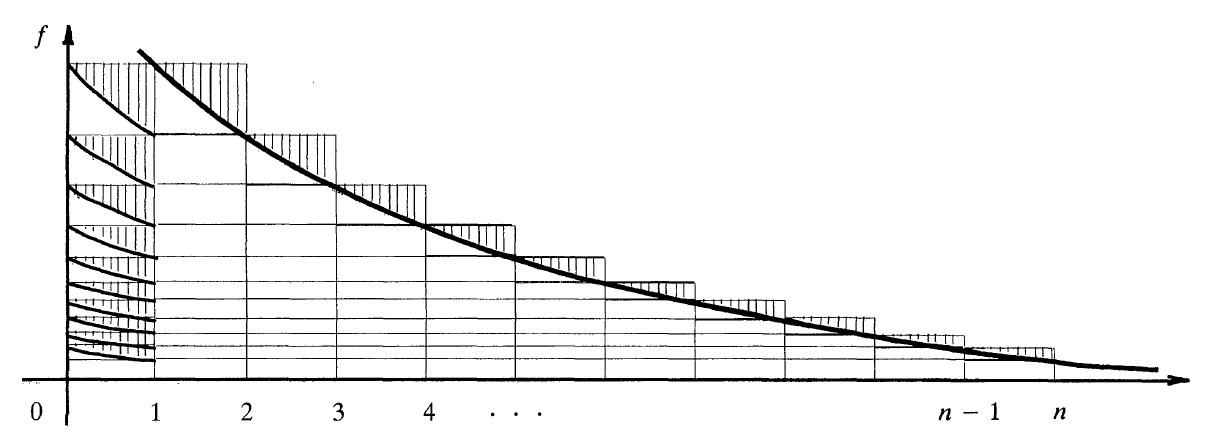
\includegraphics[width=15cm]{../image/d_n.png}
        \caption{$d_n$的几何解释}
        \label{fig: d_n的几何解释}
      \end{figure}
      \figref{fig: d_n的几何解释}为$d_n$的几何解释,其中
      在曲线上方的阴影部分即为$d_n$,可以将它们统一移动到图像的最左侧.

    \begin{defi}[广义Euler常数]
      已知$0<d_n<d_{n+1}<\f(1)$,所以可以定义关于$\f$的广义Euler常数
      $C(\f)$为
      \[
        C(\f) = \lim_{n\to\infty}d(n)
      \]
    \end{defi}

    \begin{pos}[余项估计]
      $0 < C(\f) - d_n < \f(n)$.
    \end{pos}

    \begin{thm}
      设$\f$在$[1,\infty)$上为正且严格单调递减,则存在一列
      $\{E_{\f}(n)\}$,满足$0<E_{\f}(n) < \f(n)$,成立
      \begin{equation}
        \sum_{k=1}^n\f(k) = \int_1^n\f\rd x + C(\f) + E_{\f}(n),
        \quad n = 2,3,\dots.
      \end{equation}
    \end{thm}
    \remark
      只需令$\lhs = \sum_{k=1}^{n-1}\f(k) + \f(n)$,在根据$d_n$
      的定义即可证明. 这一定理意味着求和与积分之间的误差仅仅为一个与
      $\f$有关的常数以及一个比$\f(n)$还要小的正数. 从而如果$\f(n)\to 0$,
      则$E_{\f}(n)\to 0$,此时成立
      \begin{equation}
        C(\f) = \lim_{n\to\infty}\left(
          \sum_{k=1}^n \f(k) - \int_1^n\f(x)\rd x
        \right).
      \end{equation}

    \begin{defi}[经典Euler常数]
      取$\f(x) = 1/x$,它满足$\lim_{x\to\infty}\f(x) = 0$,则有
      \[
        \gamma = C(\frac{1}{x}) = \lim_{n\to\infty}\left(
          \sum_{k=1}^n\frac{1}{k} - \ln n
        \right).
      \]
    \end{defi}

  \subsubsection{Euler求和公式}
    \paragraph{绪论}
      在此章节不再限制$\f$需要为正且单调减,在目前仅要求$\f\in\ms{R}[1, n]$
      (在之后会添加诸如连续可导等条件). 在此基础上重新定义$d_n$(与上一节保持一致)
      并推导出类似于上一节中的结论.

    \begin{defi}[$d_n$]
      定义$d_n$为
      \begin{equation}
        d_n = \sum_{k=1}^{n-1}I(k) =
        \sum_{k=1}^{n-1} \int_{k}^{k+1}\{ \f(k) - \f(x) \}\rd x.
      \end{equation}
    \end{defi}
    \remark
      可以发现这一定义和上一节中的定义,在$\f>0$且单调减的情况下是一致的.
      实际上这一定义只是将每一点处的差值积分起来而已.

    \begin{pos}
      对于任意常数$c$,由于成立$\rd x= \rd(x+c)$,所以可以取$c=-(k+1)$,并分部
      积分,则有
      \[
        I(k) = \int_{k}^{k+1} (x-[x]-1)\f\hp(x)\rd x.
      \]
      从而
      \[
        d_n = \int_1^n(x-[x])\f\hp(x)\rd x + \f(1) - \f(n).
      \]
    \end{pos}

    \begin{thm}[一次导数形式的Euler求和公式]
      对于任意$\f\in\ms{C}^1[1,n]$,成立
      \begin{equation}
        \label{equ: 一次导数Euler求和公式}
        \sum_{k=1}^n\f(k) = \int_1^n\f(x)\rd x +
        \int_1^n(x-[x])\f\hp(x)\rd x + \f(1).
      \end{equation}
    \end{thm}
    \remark
      对于误差项中的$\f\hp$,如果它不变号,即$\f$单调的情况下,
      可以考虑让它乘一个变号的因数,从而使得误差更小. 例如,可以
      用$x-[x]-\frac{1}{2}$来代替$x-[x]$. 则有了如下推论.

    \begin{cor}
      \label{cor: 一次Euler求和公式}
      对于任意$\f\in\ms{C}^1[1,n]$,定义一次Bernoulli函数为
      \[
        P_1(x) =
        \begin{cases}
          x - [x] - \frac{1}{2},\quad& x \notin \mbf{N} \\
          0, & x\in\mbf{N}.
        \end{cases}
      \]
      则可以重写\equref{equ: 一次导数Euler求和公式}为
      \begin{equation}
        \sum_{k=1}^n\f(k) = \int_1^n\f(x)\rd x +
        \int_1^nP_1(x)\f\hp(x)\rd x + \frac{1}{2}(\f(n) + \f(1)).
      \end{equation}
      若假设$\int_1^{\infty}P_1\f\rd x$存在,那么上式可以继续写为
      \[
        \begin{split}
        \sum_{k=1}^n\f(k) &= \int_1^n\f(x)\rd x + C(\f) + E_{\f}(n) \\
        C(\f) &= \frac{1}{2}\f(1) + \int_1^{\infty}P_1\f\hp\rd x\\
        E_{\f}(n) &= \frac{1}{2}\f(n) - \int_n^{\infty}P_1\f\hp\rd x
      \end{split}\]
    \end{cor}
    \remark
      注意,在此处$C(\f)$和$E_{\f}(n)$的定义和之前依然是一致的. 并且只需要
      $\f(x)$在$[1, \infty)$上反常绝对可积,就可以保证
      $\int_1^\infty P_1\f\rd x$的存在性.\footnote{我暂时并没有明白,是
      什么条件保证了$\f(n)\to 0$,从而$C(\f) = \lim_{n\to\infty}d_n$存在.}

    \begin{cor}[Euler常数]
      将$\f(x) = 1/x$,代入\corref{cor: 一次Euler求和公式},得
      经典Euler常数$\gamma$为
      \[
        \gamma = \frac{1}{2} = \int_1^\infty \frac{P_1(x)}{x}\rd x.
      \]
    \end{cor}

  \subsubsection{余项分析}
    \paragraph{绪论}
      这一章节通过对
      \begin{equation}
        \label{equ: Euler求和公式余项1}
        \int_n^{n+1}P_1(x)\f(x)\rd x
      \end{equation}
      分部积分来进一步分析余项,并为此引入了更高次的Bernoulli函数.

    \begin{defi}[二次Bernoulli函数]
      定义二次Bernoulli函数$P_2(x)$为
      \[
        P_2(x) = 2\int_0^xP_1(t)\rd t + \frac{1}{6}.
      \]
    \end{defi}
    \remark
      如此定义二次Bernoulli函数的动机来自于对
      \equref{equ: Euler求和公式余项1}的进一步分部积分. 这样就需要有
      \[
        P_2(x) = 2\int_0^xP_1(t)\rd t + c
      \]
      之所以要有系数$2$是为了之后公式的简洁. 由于$P_1(x)$有周期性,从而
      \[
        P_2(x+1) - P_2(x) = 2\int_x^{x+1}P_1(t)\rd t = 0,
      \]
      即$P_2(x)$也有周期性. 为了让按照同样方式定义的$P_3$也具有周期性,
      所以希望有
      \[
        \int_0^1P_2(x)\rd x= 0 \,\Rightarrow\, c = \frac{1}{6}.
        \quad\blacksquare
      \]

    \begin{thm}[二次导数形式的Euler求和公式]
      设$\f\in\ms{C}^2[1, n]$,成立
      \[
        \sum_{k=1}^n\f(k) = \int_1^n\f\rd x
        - \frac{1}{2}\int_1^nP_2\f^{\pr\pr}\rd x
        + \frac{1}{2}P_2(0)(\f\hp(n)-\f\hp(1))
        + \frac{1}{2}(\f(n) + \f(1)).
      \]
      并且,如果$\f^{\pr\pr}$在$[1, \infty)$上反常绝对可积,则有
      \[\begin{split}
        \sum_{k=1}^n\f(k) &= \int_1^n\f\rd x + C(\f) + E_{\f}(n) \\
        C(\f) &= \frac{1}{2}\f(1) - \frac{1}{2}P_2(0)\f\hp(1)
        - \frac{1}{2}\int_1^\infty P_2\f^{\pr\pr}\rd x \\
        E_{\f}(n) = \frac{1}{2}\f(n) + \frac{1}{2}P_2(0)\f\hp(n) +
        \frac{1}{2}\int_n^\infty P_2\f^{\pr\pr}\rd x.
      \end{split}\]
    \end{thm}

  \subsubsection{Bernoulli数和Euler求和公式的一般形式}
    \begin{defi}
      定义\tbf{Bernoulli周期函数}为
      \begin{equation}
          P_k(x) = k\int_0^x P_{k-1}(t)\rd t + B_k,\quad k\ge 2
      \end{equation}
      其中$B_k$称为\tbf{Bernoulli数},它使得下式成立
      \[
        \int_0^1P_k(x)\rd x = 0.
      \]
      显然$P_k(x)$在$k\ge 2$的时候在$[0, 1]$上是$k$次多项式,称
      它为\tbf{Bernoulli多项式}.
    \end{defi}

    \begin{thm}[等价定义]
      Bernoulli数和Bernoulli多项式的另一种常见定义为,
      \[\begin{split}
        & B_0 = 1,\quad \sum_{k=0}^{m+1} {{m+1}\choose{k}} B_k = 0 \\
        & B_n(x) = \sum_{k=0}^n{{n}\choose{k}}B_{n-k}x^k.
      \end{split}\]
    \end{thm}
    \remark
      对于大于$1$的奇数$k$,$B_k=0$,且有
      \[
        |B_{2k}(x)| \le |B_{2k}|,\quad
        |B_{2k+1}(x)| \le (2k+1)|B_{2k}|.
      \]

    \begin{thm}[Euler求和公式的一般形式]
      设$\f\in\ms{C}^{2m+1}[1, n]$,成立
      \[\begin{split}
        \sum_{k=1}^n\f(k) = & \int_1^n\f\rd x +
        \frac{1}{(2m+1)!}\int_1^n P_{2m+1}(x)\f^{(2m+1)}(x)\rd x\\
        & + \sum_{r=1}^m \frac{B_{2r}}{(2r)!}(\f^{(2r-1)}(n)-\f^{(2r-1)}(1))
        + \frac{1}{2}(\f(1) + \f(n)).
      \end{split}\]
      且若$\f^{(2m+1)}$在$[1, \infty)$上反常绝对可积,则成立
      \[\begin{split}
      \sum_{k=1}^n\f(k) &= \int_1^n\f\rd x + C(\f) + E_{\f}(n) \\
      C(\f) &= \frac{1}{2}\f(1) - \sum_{r=1}^m\frac{B_{2r}}{(2r)!}\f^{(2r-1)}(1)
      + \frac{1}{(2m+1)!}\int_1^{\infty}P_{2m+1}\f^{(2m+1)}\rd x \\
      E_{\f}(n) &= \frac{1}{2}\f(n) + \sum_{r=1}^m\frac{B_{2r}}{(2r)!}\f^{(2r-1)}(n)
      - \frac{1}{(2m+1)!}\int_n^{\infty}P_{2m+1}\f^{(2m+1)}\rd x
      \end{split}\]
    \end{thm}


\end{document}
